%\section{Piégeage dipolaire dans le bleu pour des atomes de rubidium}
%\label{sec:dipoletrap}

\section*{Introduction}

Dans cette section, nous présentons l’implémentation expérimentale et théorique d’un piégeage dipolaire dans le bleu, permettant de confiner des atomes de rubidium froids à l’aide de deux barrières de potentiel. Contrairement au cas plus standard du piégeage rouge, où les atomes sont attirés vers les maxima d’intensité, un piégeage dans le bleu ($\Delta > 0$) repousse les atomes vers les minima d’intensité lumineuse, créant ainsi des barrières efficaces.

Le formalisme utilisé repose sur une description quantique du couplage dipolaire entre un champ laser classique quasi-monochromatique et un atome à deux niveaux. Nous déduisons l’Hamiltonien effectif en seconde quantification sans faire appel à des transformations de jauge. L’objectif est d’obtenir une expression exploitable pour le potentiel optique ressenti par les atomes dans le régime de grand désaccord.

% INSERTION FIGURE 2 niveaux 
\begin{figure}[!htb]
\centering
\begin{tikzpicture}
    \node[rectangle, draw = none] (exp) at (0,0) {
       \includegraphics[width=0.5\textwidth , page = 2]{Figures/Figures}
    };
%    \node[circle, draw=none, above=0cm of exp , shift={( -2.5cm , -0.5cm )} ] {(a)};
    
%    \node[right=1mm of exp , shift={( -0.5cm , 0cm )}] (pi) {
%       \includegraphics[width=0.5\textwidth , page = 4]{Figures/Figures}
%    };
%    \node[circle, draw=none, above=0cm of pi , shift={( -2.5cm , -0.5cm )}] {(b)};
\end{tikzpicture}
\caption{Structure à deux niveaux : $\ket{g}$ pour l’état fondamental ("ground") et $\ket{e}$ pour l’état excité ("excited"). La différence d’énergie entre les deux niveaux, notée $\hbar \omega_{e \rightarrow g}$, est représentée, ainsi que la transition induite par le couplage laser de fréquence $\omega$. Dans cet exemple, la transition est dans le bleu.}

\end{figure}

\vspace{1em}
% INSERTION FIGURE
\begin{center}
\textit{[Insérer ici un schéma des niveaux d’énergie du Rubidium (transitions D1 et D2, base fine)]}
\end{center}

\section{Transformation de jauge et simplification du Hamiltonien}

%(cf. Complément HIII du tome 1 de Cohen-Tannoudji)\\

\paragraph{Cadre sans potentiel vecteur.}

Soit une particule de masse $m$ couplée à un champ électromagnétique. Dans une jauge $\mathcal{J} \equiv (\operatorvec{A}, \Phi)$, le quadrivecteur potentiel s’écrit $A^\mu = \left\{ A^0 \equiv \Phi/c,\, A^i \equiv \operatorvec{A} \right\}$. Si l’on définit la dérivée covariante comme $\mathcal{D}_\mu = \partial_\mu + \frac{iq}{\hbar} A_\mu = \{ \mathcal{D}_t \equiv \partial_t + \frac{iq}{\hbar} \Phi , \operatorvec{\mathcal{D}} = \operatorvec{\nabla} - \frac{iq}{\hbar} \operatorvec{A}  \} $, l’équation de Schrödinger régissant l’évolution de la fonction d’onde $\vert \psi \rangle$  prend la forme manifestement invariante :
\begin{eqnarray*}
	i\hbar \mathcal{D}_t \vert \psi \rangle = \frac{1}{2m} \left( \frac{\hbar}{i} \operatorvec{\mathcal{D}} \right)^2 \vert \psi \rangle, & soit &  i\hbar \partial_t \vert \psi \rangle = H_{\mathcal{J}} \vert \psi \rangle , ~\mbox{avec}~	H_{\mathcal{J}} = \frac{1}{2m} (\operatorvec{P} - q \operatorvec{A})^2 + q\Phi
\end{eqnarray*}


\paragraph{Hamiltonien simplifié.}

Dans une autre jauge $\mathcal{J}'$, le potentiel s’écrit $A'^\mu = \{ \Phi'/c,\, \operatorvec{A}' \}$ avec $ A'_\mu = A_\mu - \partial_\mu \chi$, où $\chi$ est une fonction scalaire dépendant de l’espace et du temps. Un argument rapide pour garantir que cette transformation conserve les équations de Maxwell est que le tenseur électromagnétique
\(
F_{\mu\nu} = \partial_\mu A_\nu - \partial_\nu A_\mu
\)
est invariant par changement de jauge. Dans cette nouvelle jauge , la dérivé corariante s'écrit $\mathcal{D}_\mu' = \partial_\mu + \frac{iq}{\hbar} A_\mu' = \{ \mathcal{D}_t' \equiv \partial_t + \frac{iq}{\hbar} ( \Phi - \partial_t \chi )   , \operatorvec{\mathcal{D}}' \equiv \operatorvec{\nabla} - \frac{iq}{\hbar} (\operatorvec{A} + \operatorvec{\nabla}\chi)\} $, l’équation de Schrödinger s'écrit
\begin{eqnarray*}
	i\hbar \mathcal{D}_t' \vert \psi' \rangle = \frac{1}{2m} \left( \frac{\hbar}{i} \operatorvec{\mathcal{D}}' \right)^2 \vert \psi' \rangle, & soit &  i\hbar \partial_t \vert \psi' \rangle = H_{\mathcal{J}'} \vert \psi' \rangle , ~\mbox{avec}~	H_{\mathcal{J}'} = -q\partial_t \chi + \tilde{H}_{\mathcal{J}},% \frac{1}{2m} (\operatorvec{P} - q \operatorvec{A})^2 + q\Phi
\end{eqnarray*}
avec $\vert \psi'\rangle = \operator{T}_\chi(t) \vert \psi\rangle$, $\operator{T}_\chi(t) \equiv \exp\left( \frac{iq}{\hbar} \chi(\operatorvec{R}, t) \right)$ et $\tilde{H}_{\mathcal{J}} = \operator{T}_\chi H_{\mathcal{J}}\operator{T}_\chi^\dag = \frac{1}{2m} ( \operatorvec{P} - q  ( \operatorvec{A} + \operatorvec{\nabla}\chi  )  )^2 + q \Phi $. Je choisie $\chi = - \operatorvec{R}\cdot\operatorvec{A}$ (ie $\mathcal{J}' \equiv (\operatorvec{A})$). $\operator{T}_\chi(t)$ devient un operateur translation de $iq \operatorvec{A}$ dans l’espace des impultion , et l'opérateur champs électrique transverse étant $\operatorvec{E}_\perp = - \partial_t \operatorvec{A}$. L'Hamiltonien $H_{\mathcal{J}'}$ devient :
\begin{eqnarray*}
	\operator{H}_{\mathcal{J}'} & = & 	\tilde{\operator{H}}_{\mathcal{J}}	+ \operator{H}_{\text{int}},
\end{eqnarray*}
avec $\tilde{H}_{\mathcal{J}} = \frac{1}{2m}\operatorvec{P}^2 +q \Phi$. L’opérateur de couplage atome-rayonnement quantifié est donné par :
\(
\operator{H}_{\text{int}} = - \operatorvec{D} \cdot \operatorvec{E}_\perp,
\)
où \(\operatorvec{D}\) est l’opérateur de moment dipolaire électrique, défini par :
\(
\operatorvec{D} = q \operatorvec{R}.
\)



\paragraph{Conclusion – Simplification par transformation de jauge}
\bigskip
%\begin{tcolorbox}[colback=gray!10, colframe=black, title=Conclusion]
La transformation de jauge que nous avons appliquée permet de travailler dans un cadre où le{\bf  potentiel vecteur} est nul. Dans cette jauge particulière, le Hamiltonien du système est considérablement simplifié, car le couplage au champ électromagnétique ne se fait plus par le terme de couplage minimal \((\operatorvec{P} - q \operatorvec{A})^2\), mais uniquement à travers un {\bf potentiel scalaire effectif}.

Cette simplification rend l’analyse théorique plus accessible et facilite l’interprétation physique du rôle du champ électromagnétique, en le ramenant à une simple modulation de l’énergie potentielle.
%\end{tcolorbox}




\section{Potentiel Dipolaire d'un atome à deux niveaux - généralité}

\subsection{Introduction.}
Un atome neutre placé dans un champ électrique $\operatorvec{E}_\perp$ développe un moment dipolaire induit $\operatorvec{D}(t)$. Si le champ varie lentement devant la dynamique interne de l’atome, le moment dipolaire reste aligné avec la composante transverse du champ, $\operatorvec{E}_\perp(t)$, et l’énergie potentielle d’interaction s’écrit 
\(
 \operator{H}_{\text{int}}(t) = -\operatorvec{D}(t) \cdot \operatorvec{E}_\perp(t).
\)

Dans cette configuration, l’énergie potentielle est minimale là où l’intensité du champ est maximale. L’atome est alors attiré vers les régions de forte intensité du champ électrique : on parle de \textit{piège dipolaire optique}, ou encore de \textit{pince optique}.

% INSERTION FIGURE 2 niveaux 
\begin{figure}[!htb]
\centering
\begin{tikzpicture}
    \node[rectangle, draw = none] (exp) at (0,0) {
       \includegraphics[width=0.5\textwidth , page = 2]{Figures/Figures}
    };
%    \node[circle, draw=none, above=0cm of exp , shift={( -2.5cm , -0.5cm )} ] {(a)};
    
%    \node[right=1mm of exp , shift={( -0.5cm , 0cm )}] (pi) {
%       \includegraphics[width=0.5\textwidth , page = 4]{Figures/Figures}
%    };
%    \node[circle, draw=none, above=0cm of pi , shift={( -2.5cm , -0.5cm )}] {(b)};
\end{tikzpicture}
\caption{Structure à deux niveaux : $\ket{g}$ pour l’état fondamental ("ground") et $\ket{e}$ pour l’état excité ("excited"). La différence d’énergie entre les deux niveaux, notée $\hbar \omega_{e \rightarrow g}$, est représentée, ainsi que la transition induite par le couplage laser de fréquence $\omega$. Dans cet exemple, la transition est dans le bleu.}

\end{figure}


\subsection{Système à deux niveaux et interaction avec le champ.}


Considérons un atome modélisé par deux états, le fondamental $\ket{g}$ d'énergie $\hbar \omega_g$  et l’excité $\ket{e}$ d'énergie $\hbar \omega_e$, couplés par le champ électrique $\operatorvec{E}_\perp(\vec{r} , t ) = \operatorvec{\mathcal{E}}(\vec{r}) \cos ( \omega t )  $. le champ laser est loin de la résonance avec l’état excité $\ket{e}$ , c’est-à-dire que le désaccord $\Delta = \omega - \omega_{e\rightarrow g}$ (avec la fréquence de transition $\omega_{g\rightarrow e} = \omega_e - \omega_g $ ) est grand comparé à la fréquence de Rabi définissant le couplage entre le dipôle et le champ 
\[\Omega(\vec{r}) = -  \bra{e} \operatorvec{D} \cdot \operatorvec{\mathcal{E}}(\vec{r}) \ket{g}/\hbar = - \vec{d}_{g\leftrightarrow e } \cdot  \vec{\mathcal{E}}(\vec{r}) /\hbar,
\] avec $\vec{d}_{g\leftrightarrow e } = \bra{e} \operatorvec{D} \ket{g} $ l’élément de matrice dipolaire réel entre $\ket{g}$ et $\ket{g}$. 

\vspace{1em}
% INSERTION FIGURE
\begin{center}
\textit{[Insérer ici un schéma des niveaux d’énergie du Rubidium (transitions D1 et D2, base fine)]}
\end{center}

\subsection{Interprétation du traitement du second ordre : transition virtuelle et origine du potentiel dipolaire (AC-Stark)}

\paragraph{Transition virtuelle et suppression des transitions réelles.}
Lorsque le champ laser est fortement dé-tuné par rapport à la résonance atomique, c’est-à-dire que le désaccord \( \Delta = \omega - \omega_{g\rightarrow e} \) vérifie \( |\Delta| \gg \Gamma \), l’excitation réelle de l’atome devient négligeable. En effet, le paramètre \( \Gamma \) désigne la \emph{largeur naturelle} de la transition \( \ket{e} \rightarrow \ket{g} \), c’est-à-dire le taux d’émission spontanée d’un photon par un atome excité. Elle est liée à la durée de vie \( \tau \) de l’état \( \ket{e} \) par \( \Gamma = 1/\tau \), et  dans le cas d’une transition dipolaire électrique  peut être calculée à partir de l’électrodynamique quantique selon la formule :
\begin{equation}
	\Gamma = \frac{\omega_{e\rightarrow g}^3}{3 \pi \varepsilon_0 \hbar c^3} |\vec{d}_{e \leftrightarrow g } |^2,
\end{equation}

où \( \varepsilon_0 \) est la permittivité du vide, et \( c \) la vitesse de la lumière.\\La probabilité d’exciter réellement l’atome vers l’état \( \ket{e} \) devient négligeable : le champ ne peut pas induire une véritable transition \( \ket{g} \to \ket{e} \).\\


\bigskip

\paragraph{Effet de second ordre : origine du potentiel dipolaire.}

\noindent Toutefois, même si le champ laser ne permet pas de peupler réellement l’état excité, il peut induire des transitions \emph{virtuelles} via l’interaction dipolaire \(  \operator{H}_{\text{int}} \). Le système passe temporairement par l’état \( \ket{e} \) sans s’y stabiliser :
\[
\ket{g} \xrightarrow{\quad \operator{H}_{\text{int}} \quad} \ket{e} \xrightarrow{\quad \operator{H}_{\text{int}} \quad} \ket{g},
\]
Ce processus modifie l’énergie propre de l’état \( \ket{g} \), générant un \textbf{décalage AC-Stark}, interprété comme un \emph{potentiel dipolaire}.


Ce phénomène s’interprète naturellement comme un effet de second ordre en théorie des perturbations indépendantes du temps. La correction d’énergie associée à l’état \( \ket{g} \) s’écrit :

\begin{equation}
\delta E_g^{(2)} =  \frac{|\bra{e} \operator{H}_{\text{int}} \ket{g}|^2}{\hbar \Delta}.
\end{equation}
Cette correction est responsable de l’apparition d’un potentiel effectif ressenti par l’atome, appelé \emph{potentiel dipolaire optique}.


\bigskip

\paragraph{Analyse perturbative à différents ordres :}

\begin{itemize}[label = $\bullet$] 
\item \textbf{Ordre 0} — énergie non perturbée :  
L’atome est dans l’état fondamental \( \ket{g} \). Son énergie propre est simplement :  
\[
E_g^{(0)} = E_g.
\]

\item \textbf{Ordre 1} — pas de correction diagonale :  

Dans l’approximation des grandes longueurs d’onde \( \lambda \gg \langle \vec{r} \rangle \), c’est-à-dire lorsque la longueur d’onde du champ laser est grande devant la taille de l’atome, l’interaction lumière-matière se décrit par le \emph{Hamiltonien dipolaire électrique} . Dans ce cadre, la correction d’énergie au premier ordre est donnée par :
\[
\delta E_g^{(1)} = \bra{g} \operator{H}_{\text{int}} \ket{g}.
\]

Or, pour un champ oscillant typiquement de la forme \( \vec{E}_{\perp}(t) = \frac{1}{2} \vec{\mathcal{E}}\, e^{-i\omega t} + \text{c.c.} \), ce terme est rapide et oscille à la fréquence du laser. De plus, dans une base d’états propres de parité définie (comme c’est le cas pour les niveaux atomiques), l’opérateur \( \operatorvec{D} \) étant de parité impaire, son \textbf{élément diagonal est nul} :

\[
\bra{g}  \operatorvec{D} \ket{g} = 0 \quad \Rightarrow \quad \bra{g} \operator{H}_{\text{int}} \ket{g} = 0.
\]

Ainsi, non seulement \( \delta E_g^{(1)}(t) \sim \cos(\omega t) \) est une oscillation à haute fréquence, mais sa moyenne temporelle est aussi nulle :
\[
\langle \delta E_g^{(1)} \rangle_t = 0.
\]

Par conséquent, il n’y a \textbf{aucun décalage d’énergie net à l’ordre 1} : c’est uniquement à l’ordre 2 que l’interaction induit un potentiel stationnaire, correspondant au déplacement AC-Stark.


\item \textbf{Ordre 2} — transition virtuelle :  
On applique alors la théorie des perturbations au second ordre, ce qui donne la correction :

\begin{equation}
\delta E_g^{(2)} =  \frac{|\bra{e} \operator{H}_{\text{int}} \ket{g}|^2}{\hbar \Delta},
\end{equation}

Cette correction donne lieu à un \emph{potentiel effectif} ressenti par l’atome dans son état fondamental, appelé \textbf{potentiel dipolaire optique}.
\end{itemize}

\bigskip

\subsection{Expression explicite du potentiel dipolaire}

\subparagraph{Champ électrique appliqué.}
On considère un champ électrique de la forme :
\begin{equation}
\vec{E}_\perp(\vec{r},t) = \frac{1}{2} \vec{\mathcal{E}}(\vec{r}) \, e^{-i\omega t} + \text{c.c.}, \quad \mbox{avec}  \, \vec{\mathcal{E}}(\vec{r}) =  {\mathcal{E}}(\vec{r})\, \vec{u}
\end{equation}
où \( \vec{u} \) est un vecteur de polarisation unitaire, et \( {\mathcal{E}}(\vec{r}) \) est l’amplitude complexe spatiale du champ.


\paragraph{Potentiel dipolaire}.
La correction d’énergie à l’ordre 2 s’écrit alors :
\begin{equation}
	U_{\mathrm{dip}}(\vec{r}) = \delta E_g^{(2)} = \frac{\hbar \, \Omega^2(\vec{r})}{4 \Delta},\label{eq:Udip1}
\end{equation}
et en exprimant la fréquence de Rabi \( \Omega \) via \( \Gamma \) et \( I_{\mathrm{sat}} \), on obtient la forme opérationnelle suivante du potentiel :
\begin{equation}
	U_{\mathrm{dip}}(\vec{r}) = \frac{\hbar \Gamma^2}{8 I_{\mathrm{sat}}} \cdot \frac{I(\vec{r})}{\Delta},
	\label{eq:Udip2}
\end{equation}
où : \( I(\vec{r}) = \frac{1}{2} \varepsilon_0 c |\vec{\mathcal{E}}(\vec{r})|^2\) est l’intensité locale du champ laser et \( I_{\mathrm{sat}}  = \frac{\hbar \omega_{e \rightarrow g}^3 \Gamma}{12 \pi c^2}\) est l’intensité de saturation.


Cette forme montre que le potentiel dipolaire est proportionnel à l’intensité lumineuse locale. 


Ce potentiel permet de décrire le confinement des atomes dans des régions où \( I(\vec{r}) \) est élevé (ou faible, selon le signe de \( \Delta \)), formant ainsi des barrières optiques contrôlables avec une résolution sub-micronique.


\subparagraph{Conditions de validité.}

Les expressions~\eqref{eq:Udip1} et \eqref{eq:Udip2}  pour le potentiel dipolaire est obtenue sous les hypothèses suivantes, qui assurent la validité du modèle à deux niveaux et du traitement perturbatif :

\begin{itemize}[label = $\bullet$]
  \item \textbf{Réduction à un sous-espace résonant} : le champ est quasi-résonant avec une seule transition atomique, ce qui suppose que le désaccord est faible devant les fréquences optiques impliquées, i.e. $|\Delta| \ll \omega, \omega_{\scriptstyle g \rightarrow e}$. Cela permet de restreindre le système à deux niveaux et d’ignorer les autres transitions dipolaires.
  
  \item \textbf{Régime de grand désaccord en fréquence (large détuning)} : lorsque $|\Delta| \gg \Gamma$, c’est-à-dire lorsque le désaccord est grand devant la largeur naturelle de la transition, les excitations réelles vers l’état excité sont fortement supprimées. L’interaction lumière-matière peut alors être traitée en perturbation du second ordre : l’atome reste majoritairement dans son état fondamental, et l’effet du champ lumineux se manifeste sous la forme d’un potentiel effectif induit par des couplages virtuels.
  
  \item \textbf{Régime de faible saturation} : on suppose que la fréquence de Rabi $\Omega$ est beaucoup plus faible que le désaccord, i.e. $\Omega \ll |\Delta|$. Cette condition garantit que la population de l’état excité reste négligeable, ce qui justifie l’approximation adiabatique sur l’état fondamental.
\end{itemize}


%\subparagraph{Conditions de validité}

%L’expression~\eqref{eq:Udip} repose sur les hypothèses suivantes :
%\begin{itemize}
%  \item $|\Delta| \ll \omega_L, \omega_{5P5S}$ : validité du modèle à deux niveaux ;
%  \item $|\Delta| \gg \Gamma$ : justification de l’approximation perturbative ;
%  \item $\Omega \ll |\Delta|$ : régime de faible saturation.
%\end{itemize}

%\subparagraph{Régime de grand désaccord en fréquence (détuning).}

%Dans le cas où le désaccord \(\Delta = \omega_L - \omega_{5P5S}\) est grand devant le taux de décroissance radiative \(\Gamma\), c’est-à-dire lorsque \(|\Delta| \gg \Gamma\), l’interaction avec le champ lumineux peut être traitée en perturbation du second ordre. Cette approche permet de projeter l’effet du champ lumineux sur l’état fondamental de l’atome, en négligeant les transitions réelles vers l’état excité.


\subparagraph{Interprétation physique.}

Le potentiel \( U_{\mathrm{dip}}(\vec{r}) \) représente une énergie potentielle effective induite par l’interaction entre un atome neutre et le champ laser. Il dépend explicitement de la position \( \vec{r} \) via l’intensité locale du champ lumineux \( I(\vec{r}) \). Ce potentiel guide ainsi la dynamique de l’atome comme le ferait un potentiel externe classique.

La direction du mouvement dépend du signe du désaccord \( \Delta = \omega - \omega_{e \rightarrow g} \) :

\begin{itemize}[label =$\bullet$]
  \item Si \( \Delta < 0 \) (désaccord rouge), le potentiel est attractif : les atomes sont attirés vers les zones de forte intensité lumineuse.
  \item Si \( \Delta > 0 \) (désaccord bleu), le potentiel est répulsif : les atomes sont repoussés vers les régions de faible intensité.
\end{itemize}

Ce phénomène est à la base des pièges dipolaires optiques, largement utilisés dans les expériences de refroidissement et de confinement d’atomes ultrafroids.


%\subparagraph{Confinement optique.}

%Ce potentiel dipolaire peut être utilisé pour piéger des atomes neutres. En focalisant le faisceau laser, on crée une variation spatiale de l’intensité lumineuse, et donc du potentiel dipolaire. Cela permet de construire des pièges optiques ou des réseaux d’interférences lumineuses appelés « réseaux optiques », où les atomes peuvent être confinés et manipulés avec une grande précision.

\subparagraph{Confinement optique.}

Le potentiel dipolaire \( U_{\mathrm{dip}}(\vec{r}) \), dépendant de la position via l’intensité du champ laser, permet de confiner des atomes neutres en créant des paysages de potentiel contrôlés. Selon la géométrie du champ lumineux, on peut générer des régions de potentiel attractif ou répulsif.

Dans le cas d’un désaccord bleu (\( \Delta > 0 \)), les atomes sont repoussés des zones de forte intensité. On peut alors façonner des \textit{barrières de potentiel} en structurant l’intensité lumineuse, par exemple à l’aide de faisceaux interférents ou d’optiques diffractives. Cela permet de créer des cavités, des guides ou des réseaux où les atomes sont confinés entre les zones lumineuses, sans nécessairement focaliser le faisceau.


%\subparagraph{Taux de diffusion spontanée.}
%
%L’interaction avec le champ lumineux conduit à une absorption suivie d’une réémission spontanée. Le taux de diffusion dans le régime précédent est :
%\begin{eqnarray}
%\Gamma_{\mathrm{sp}}(\operatorvec{r}) = \frac{\Gamma \, \Omega^2(\operatorvec{r})}{4 \Delta^2}
%= \frac{\Gamma^3}{8 I_{\mathrm{sat}}} \cdot \frac{I(\operatorvec{r})}{\Delta^2}.
%\label{eq:GammaSp}
%\end{eqnarray}

\subparagraph{Diffusion spontanée résiduelle.}

Un autre aspect important de l’interaction lumière-matière est la diffusion spontanée induite par le champ lumineux. Même lorsque le champ est fortement dé-tuné et que l’état excité n’est que virtuellement peuplé, une faible probabilité de transition réelle subsiste. Elle conduit à l’émission spontanée de photons, accompagnée d’un transfert aléatoire d’impulsion à l’atome, ce qui génère un chauffage du nuage atomique.

Le taux de diffusion spontanée dans le régime dispersif s’écrit :
\begin{eqnarray}
\Gamma_{\mathrm{sp}}(\operatorvec{r}) = \frac{\Gamma \, \Omega^2(\operatorvec{r})}{4 \Delta^2}
= \frac{\Gamma^3}{8 I_{\mathrm{sat}}} \cdot \frac{I(\operatorvec{r})}{\Delta^2}.
\label{eq:GammaSp}
\end{eqnarray}

Il est donc crucial, pour limiter le réchauffement, de travailler à fort désaccord \( |\Delta| \gg \Gamma \), tout en maintenant une intensité suffisante pour produire un potentiel dipolaire profond.


%\subparagraph{Bilan — compromis intensité / désaccord}
%
%Les expressions~\eqref{eq:Udip} et~\eqref{eq:GammaSp} révèlent un compromis fondamental : Le potentiel varie comme $I / \Delta$ ; Le taux de diffusion varie comme $I / \Delta^2$.
%Pour minimiser les pertes par diffusion tout en conservant un potentiel significatif, il est donc optimal d’utiliser un désaccord important avec une intensité élevée. %Ce régime est appelé \textit{FORT} (Far-Off Resonance Optical Trap).

\subparagraph{Optimisation du régime dispersif pour un potentiel donné.}

À partir des expressions~\eqref{eq:Udip2} et~\eqref{eq:GammaSp}, on peut analyser comment minimiser le taux de diffusion spontanée \( \Gamma_{\mathrm{sp}} \), sous la contrainte de produire un potentiel dipolaire \( U_{\mathrm{dip}} \) fixé.

On observe en effet que :
\[
U_{\mathrm{dip}}(\vec{r}) \propto \frac{I(\vec{r})}{\Delta}, \quad \text{tandis que} \quad \Gamma_{\mathrm{sp}}(\vec{r}) \propto \frac{I(\vec{r})}{\Delta^2}.
\]

À potentiel \( U_{\mathrm{dip}} \) fixé, cela implique que :
\[
I(\vec{r}) \propto \Delta \quad \Rightarrow \quad \Gamma_{\mathrm{sp}}(\vec{r}) \propto \frac{1}{\Delta}.
\]

Autrement dit, pour produire un potentiel donné, le taux de diffusion diminue linéairement avec \( |\Delta| \). Il est donc avantageux de travailler à grand désaccord : plus \( \Delta \) est grand, plus l’intensité requise est élevée, mais moins le taux de diffusion est important.

Ce raisonnement montre que l’on n’a pas véritablement un « compromis » entre \( I \) et \( \Gamma_{\mathrm{sp}} \), mais plutôt une {\em stratégie optimale} : à potentiel fixé, augmenter le désaccord est toujours bénéfique vis-à-vis du chauffage.


\section{Piégeage dipolaire d’un atome à plusieurs niveaux}

\subsection{Atomes multiniveaux et origine du potentiel dipolaire dans le formalisme quantique}

Le modèle à deux niveaux est suffisant pour introduire le concept de piégeage dipolaire, mais il reste limité pour décrire les détails réels d'un atome comme le \({}^{87}\mathrm{Rb}\), qui possède une structure hyperfine et fine complexe. Dans ce contexte, le potentiel dipolaire dépend du sous-niveau quantique occupé par l’atome, et le traitement doit être généralisé.

\subsubsection{Description quantique de l’atome et du champ laser}

Considérons un atome immobile possédant un état fondamental \( \ket{g} \) et une série d’états excités \( \ket{e_i} \), d’énergies respectives \( \hbar\omega_g \) et \( \hbar\omega_i \). Le champ laser est quantifié dans un volume \( V \), polarisé selon \( \vec{u} \), et d'expression 
\[
\operatorvec{E}_\perp(t) = \operator{\mathcal{E}} \vec{u} \cos(\omega t) \quad \longrightarrow \quad \operator{E}_\perp = \sqrt{\frac{\hbar \omega}{2\varepsilon_0 V}} \, \vec{u} \, (\operator{a} + \operator{a}^\dagger),
\]
où \( \operator{a} \) et \( \operator{a}^\dagger \) sont les opérateurs d’annihilation et de création de photons à la fréquence \( \omega \).

L’hamiltonien total du système « atome + champ » s’écrit alors :
\[
\operator{H} = \operator{H}_{\mathrm{at}} + \operator{H}_{\mathrm{L}} + \operator{H}_{\mathrm{int}},
\]
dans le formalisme {\bf atome + champ quantifié}, aussi appelé {\bf formalisme de l’atome habillé} , avec :
\begin{itemize}[label = $\bullet$]
	\item \(\operator{H}_{\mathrm{at}} = \sum_i \hbar \omega_i \ket{e_i}\bra{e_i} \) l’hamiltonien de l’atome. Il décrit les états propres internes (typiquement les niveaux électroniques) sans interaction avec le champ. Ici, chaque état excité $\ket{e_i}$ est associé à une énergie $\hbar \omega_i$;
	\item \(\operator{H}_{\mathrm{L}} = \hbar \omega \left(\operator{a}^\dagger \operator{a} + \frac{1}{2}\right)\) l’hamiltonien du {\bf champ électromagnétique quantifié} dans un mode unique (celui du laser). Il est représenté comme un oscillateur harmonique quantique avec énergie $ \hbar \omega $  par photon, et opérateurs \( \operator{a} \) , \( \operator{a}^\dagger \) de création/annihilation de photons. Le terme $\tfrac12 \hbar \omega $est l’énergie du vide (qui peut être ignorée dans la plupart des cas);
	\item $\operator{H}_{\mathrm{int}} = - \operatorvec{D} \cdot \operatorvec{E}_\perp$ : interaction \textbf{dipolaire quantifiée} entre l’atome et le champ électrique transverse $\operatorvec{E}_\perp$.L’Hamiltonien décrivant cette interaction, dans l’\textit{approximation des grandes longueurs d’onde} ($\lambda \gg \langle \vec{r} \rangle$, où $\vec{r}$ est la position relative de l’électron par rapport au noyau), prend la forme de l’\textbf{Hamiltonien dipolaire électrique}~\cite{CohenTannoudjiPhotonsAtomes, SteckRubidium87}. L’opérateur de moment dipolaire atomique $\operatorvec{D}$ s’écrit :
\(
\operatorvec{D} = \sum_{e_i} \vec{d}_{g \rightarrow e_i} \ket{g} \bra{e_i} + \text{h.c.}
\)
où $\vec{d}_{g \rightarrow e_i} = \bra{g} \operatorvec{D} \ket{e_i}$ est l’élément de matrice dipolaire entre les états $\ket{g}$ et $\ket{e_i}$, et ``h.c.'' désigne le terme hermitien conjugué. 
Cette forme exprime que seules les transitions dipolaires électriques autorisées par les règles de sélection (parité, moment angulaire) contribuent au couplage.

\end{itemize}


\subsubsection{États habillés et structure des niveaux}

Les états propres de l’Hamiltonien non-interactif \( \operator{H}_{\mathrm{at}} + \operator{H}_{\mathrm{L}} \) sont les produits tensoriels \( \ket{g, N} \) et \( \ket{e_i, N} \), décrivant un atome dans l’état \( \ket{g} \) ou \( \ket{e_i} \) avec \( N \) photons dans le mode du champ laser. Leurs énergies respectives sont \( E_g = \hbar \omega_{g} + N \hbar \omega \) et \( E_i = \hbar \omega_{e_i}  + N \hbar \omega \).

On parle d’« états habillés » pour désigner cette base atomique + champ, qui servira à construire les états propres du système complet en présence d’interaction. L’interaction dipolaire \( \operator{H}_{\text{int}} = - \operatorvec{D} \cdot \operatorvec{E}_\perp \) couple les états \( \ket{g, N+1} \) et \( \ket{e_i, N} \) via l’absorption d’un photon. Ce sont les seules transitions significatives, les autres étant très hors-résonance et négligées dans l’approximation séculaire.


\subsubsection{Traitement perturbatif et décalage d’énergie}

Le champ étant loin de la résonance avec les états \( \ket{e_i} \), on applique la théorie des perturbations indépendantes du temps au second ordre. L’interaction induit un décalage de l’énergie de l’état \( \ket{f} \) donné par :

\[
\delta E_f^{(2)} = \sum_{e_i} \frac{|\bra{e_i, N} \operator{H}_{\mathrm{int}} \ket{g, N+1}|^2}{E_i - E_g }.
\]
\subsubsection{Annulation de la correction d’énergie au premier ordre}

Dans le cadre de la théorie des perturbations indépendantes du temps, la correction d’énergie au premier ordre pour un état \( \ket{i} \) est donnée par :
\[
\delta E_i^{(1)} = \bra{i} \hat{H}_{\mathrm{int}} \ket{i}.
\]
Dans le cas de l’interaction dipolaire, l’opérateur d’interaction \( \operator{H}_{\text{int}} = - \operatorvec{D} \cdot \operatorvec{E}_\perp \) est de nature vectorielle, donc \emph{de parité impaire}. En revanche, les états électroniques \( \ket{g} \), \( \ket{e_i} \), etc., sont des états de parité définie.

Or’un opérateur de parité impaire possède des éléments diagonaux nuls dans une base d’états de parité bien définie. Ainsi :
\[
\bra{g} \operator{H}_{\text{int}}  \ket{g} = 0, \qquad \bra{e_i} \operator{H}_{\text{int}}  \ket{e_i} = 0.
\]
De manière générale, \( \operator{H}_{\text{int}}  \) ne couple que des états de parité opposée : il est donc purement hors-diagonal dans la base des états propres de \( \operator{H}_{\mathrm{at}} \).

\bigskip

\noindent Il en résulte que la correction d’énergie au premier ordre est strictement nulle :
\[
\delta E_i^{(1)} = 0.
\]
La première contribution non nulle provient donc du second ordre, qui décrit des transitions virtuelles, telles que \( \ket{g} \to \ket{e_i} \to \ket{g} \), responsables du décalage AC-Stark (ou potentiel dipolaire optique).

\subsubsection*{Approximation séculaire et sélection des transitions pertinentes}

Dans le cadre du piégeage dipolaire, nous faisons l’hypothèse que le champ laser est \textbf{quasi-résonant} avec un \textbf{nombre restreint de transitions atomiques}. Autrement dit, la fréquence du laser \( \omega \) est suffisamment proche de certaines transitions \( \omega_{g \rightarrow e_i} = \omega_{e_i} - \omega_g  \) de l’atome, de sorte que le désaccord \( \Delta_i = \omega - \omega_{g \rightarrow e_i} \) est \textbf{petit devant les fréquences optiques} elles-mêmes :
\(
|\Delta_i| \ll \omega_L, \omega_{g \rightarrow e_i}.
\)
Cette hypothèse permet de simplifier l’analyse perturbative de l’interaction atome-laser : dans la somme intervenant dans la correction d’énergie au second ordre,seuls les \textbf{termes proches de la résonance} (i.e., pour lesquels \( E_g \simeq E_i \pm \hbar \omega \)) contribuent significativement à la somme. En effet, pour ces termes, le dénominateur devient \textbf{petit}, ce qui rend leur contribution \textbf{dominante}. Les autres transitions, très éloignées en énergie, ont des dénominateurs très grands, et leur influence devient négligeable. Cette \textbf{troncature de la somme perturbative} constitue l’\textbf{approximation séculaire}.

Dans ce régime, l’interaction dipolaire sélectionne efficacement les couplages entre les états atomiques et photoniques \textbf{ayant une différence d’un seul photon} :
\[
\operator{H}_{\text{int}} : \ket{g, N+1} \longleftrightarrow \ket{e_i, N},
\]
où \( \ket{g, N+1} \) est un état fondamental avec \( N+1 \) photons, et \( \ket{e_i, N} \) un état excité \( e_i \) avec \( N \) photons.

\medskip

Dans notre cas spécifique, nous utilisons un \textbf{faisceau laser à environ 770~nm}, soit légèrement \textbf{au bleu} des raies principales du rubidium 87 :
\begin{itemize}
  \item raie \textbf{D2} : \( \lambda = 780~\text{nm} \), correspondant à la transition \( 5S_{1/2} \rightarrow 5P_{3/2} \),
  \item raie \textbf{D1} : \( \lambda = 795~\text{nm} \), correspondant à la transition \( 5S_{1/2} \rightarrow 5P_{1/2} \).
\end{itemize}

Le faisceau à environ 770~nm est donc \textbf{hors résonance}, mais \textbf{pas trop éloigné} de ces transitions (désaccord de l’ordre de quelques dizaines de THz), ce qui garantit que la structure hyperfine peut être \textbf{négligée} dans un premier temps, et que l’interaction est bien décrite par la contribution dominante des raies D1 et D2. Dans ce régime de désaccord modéré, le potentiel dipolaire est obtenu comme une somme pondérée des contributions des transitions proches, et les autres transitions atomiques (plus énergétiques) peuvent être ignorées.

\subsubsection*{Expression des éléments de matrice dans l’interaction atome-champ cohérent}

Les éléments intervenant dans l’équation de second ordre~, qui donne la correction d’énergie d’un état atomique sous l’effet du champ laser, sont des éléments de matrice du type :
\[
-\bra{e_i, N} \operatorvec{D} \cdot \operatorvec{E}_\perp \ket{g, N + 1}.
\]


\paragraph{Champ cohérent et états de Fock.} Le champ électromagnétique émis par le laser est un état \textbf{cohérent}, noté \( \ket{\alpha} \), qui est une superposition d’états de Fock \( \ket{N} \) avec une distribution de Poisson centrée autour d’une valeur moyenne \( \langle N \rangle \). Cela signifie que les composantes principales du champ se trouvent dans une bande étroite \( \Delta N \ll \langle N \rangle \). Dans cette situation, les amplitudes de transition impliquant des changements d’un seul photon, comme \( \bra{N} \operatorvec{E}_\perp \ket{N+1} \), varient très peu avec \( N \), et l’on peut faire l’approximation :
\[
\bra{N} \operatorvec{E}_\perp \ket{N+1} \approx \mathcal{E} \sqrt{N+1} \simeq \mathcal{E} \sqrt{\langle N \rangle}.
\]
Ainsi, l’élément de matrice global devient simplement proportionnel à l’amplitude classique du champ.

\paragraph{Équivalence entre champ quantique et champ classique}

Considérons un champ électromagnétique monochromatique de fréquence \( \omega \), quantifié dans un volume \( V \), contenant en moyenne \( \langle N \rangle \) photons.

\begin{itemize}[label = $\bullet$]
  \item Du point de vue quantique, l’énergie moyenne d’un champ dans un seul mode est donnée par :
  \(
  \langle \hat{H}_{\mathrm{L}} \rangle = \hbar \omega \left( \langle N \rangle + \frac{1}{2} \right).
  \)
  En négligeant l’énergie du point zéro \( \frac{1}{2} \hbar \omega \), qui ne contribue pas aux transitions physiques, on obtient :
  \[
  E_{\mathrm{quantique}} = \langle N \rangle \hbar \omega.
  \]

  \item Du point de vue classique, une onde électromagnétique de champ électrique \( \vec{E}_\perp(t) = \mathcal{E} \cos(\omega t) \vec{u} \) transporte une densité d’énergie électrique :
  \(
  u_E = \frac{1}{2} \varepsilon_0\mathcal{E}^2,
  \)
  ce qui donne une énergie totale dans le volume \( V \) :
  \[
  E_{\mathrm{classique}} = \frac{1}{2} \varepsilon_0 \mathcal{E}^2 V.
  \]
\end{itemize}

En identifiant ces deux expressions dans un seul mode, on obtient la relation fondamentale :
\[
\langle N \rangle \hbar \omega = \frac{1}{2} \varepsilon_0 \mathcal{E}^2 V,
\]
qui permet d’exprimer l’amplitude du champ électrique \( E_0 \) en fonction du nombre moyen de photons \( \langle N \rangle \) dans le champ laser.



\paragraph{Conclusion.} En conséquence, l’élément de matrice d’interaction s’écrit finalement :
\[
\bra{e_i, N} - \operatorvec{D} \cdot \operatorvec{E}_\perp \ket{g, N + 1} = - \frac{\mathcal{E}}{2} \bra{e_i} \operatorvec{D} \cdot \vec{u} \ket{g}.
\]
Ce terme relie l’état atomique \( \ket{g} \) au niveau excité \( \ket{e_i} \), avec un couplage proportionnel à l’amplitude du champ classique et à l’élément de matrice dipolaire entre les deux états. C’est ce terme qui entre au numérateur dans l’expression de la correction d’énergie au second ordre , ce qui donne lieu au potentiel dipolaire optique.\\

%{\color{blue} {\color{red} (pour d on travaille avec L)} 
%\subsubsection{Structure des états électroniques et théorème de Wigner-Eckart}
%
%Les états électroniques d’un atome sont caractérisés par des nombres quantiques liés à leur structure fine. Un état est noté \( \ket{n, J, m} \), où :
%\begin{itemize}[label = $\bullet$]
%  \item \( n \) est le nombre quantique principal, qui détermine l’énergie orbitale globale ;
%  \item \( J \) est le moment angulaire total (résultant du couplage spin-orbite \( \vec{J} = \vec{L} + \vec{S} \)) ;
%  \item \( m \in [-J, J] \) est la projection du moment angulaire total sur un axe de quantification, généralement pris comme l’axe \( z \).
%\end{itemize}
%
%L’opérateur dipolaire électrique \( \operatorvec{D} \) est une observable vectorielle, c’est-à-dire un opérateur de rang 1 au sens des tenseurs sphériques. Cela permet d’utiliser le \textbf{théorème de Wigner-Eckart} pour factoriser les éléments de matrice en une partie géométrique et une partie dynamique. Pour une transition entre deux états électroniques \( \ket{n_g, J_g, m_{J_g}} \) et \( \ket{n_e, J_e, m_{J_e}} \), l’élément de matrice dipolaire projeté sur une direction de polarisation \( \vec{\epsilon} \) s’écrit :
%
%\[
%\bra{n_e, J_e, m_{J_e}} \operatorvec{D} \cdot \vec{u} \ket{n_g, J_g, m_g} = d_{n_g J_g  \leftrightarrow  n_eJ_e} \cdot \braket{J_g, 1; m_g, q | J_e, m_e},
%\]
%
%où :
%\begin{itemize}[label =$\bullet$]
%  \item \( d_{n_g J_g  \leftrightarrow  n_eJ_e}  \) est l’élément de matrice réduit. Il ne dépend pas des projections \( m \), ni du type de polarisation, mais uniquement des orbitales atomiques et du moment angulaire total. Il contient l’information dynamique de la transition, souvent calculée ou mesurée expérimentalement.
%  \item \( \braket{J_g, 1; m_g, q | J_e, m_e} \) est un \textbf{coefficient de Clebsch-Gordan}, qui encode les règles de sélection angulaires et dépend :
%  \begin{itemize}[label =$\circ$]
%    \item de \( q = 0, \pm1 \), indexant la composante du champ selon les polarisations \( \pi \) (\( q = 0 \)) ou \( \sigma^{\pm} \) (\( q = \pm1 \)) ;
%    \item des valeurs de \( J_g, J_e \), et des projections \( m_g, m_e \).
%  \end{itemize}
%\end{itemize}
%
%Ainsi, l’amplitude de transition dépend à la fois :
%\begin{enumerate}
%  \item du couplage entre les enveloppes électroniques (contenu dans \( d_{n_g J_g  \leftrightarrow  n_eJ_e} \)) ;
%  \item de la géométrie angulaire (par la polarisation du champ et les sous-niveaux magnétiques des états).
%\end{enumerate}
%
%Ce formalisme est essentiel pour calculer précisément les amplitudes de transition et les forces dipolaires induites par un champ laser polarisé, notamment dans des atomes à structure fine/ hyperfine comme le Rubidium 87. Il permet de traiter l’ensemble des transitions atomiques pertinentes dans un gaz d’atomes refroidis et piégés, sans avoir à traiter individuellement chaque sous-niveau magnétique.
%}

\section{Cas du Rubidium 87 dans une polarisation rectiligne}

\subsection{Structure électronique du Rubidium}

L’atome de Rubidium (\textsuperscript{87}Rb) est un \textbf{élément alcalin}, c’est-à-dire qu’il possède une configuration électronique de la forme $[ \mathrm{Kr} ]\,5s^1$, avec un unique électron de valence situé dans la couche $5s$. Cela implique que la structure énergétique de l’atome est essentiellement déterminée par ce seul électron périphérique, interagissant avec un cœur atomique fermé (couche interne complète).

En première approximation, on peut donc modéliser le Rubidium comme un système à un électron, à la manière de l’atome d’hydrogène, mais avec un potentiel effectif tenant compte du blindage dû aux électrons du cœur. Ce modèle permet de comprendre la structure fine et les transitions optiques dominantes de l’atome.

La structure des niveaux d’énergie est ensuite raffinée par les effets suivants :
\begin{itemize}
  \item \textbf{Structure fine} : Elle résulte du couplage spin-orbite entre le moment angulaire orbital $\vec{L}$ et le spin $\vec{S}$ de l’électron de valence. Ce couplage divise chaque niveau orbital (par exemple, le niveau $5p$) en deux sous-niveaux caractérisés par le moment angulaire total $J = L \pm \tfrac{1}{2}$. Ainsi, la transition $5s \leftrightarrow 5p$ donne naissance aux deux raies bien connues : D1 (transition $5s_{1/2} \to 5p_{1/2}$ à 795 nm) et D2 (transition $5s_{1/2} \to 5p_{3/2}$ à 780 nm).
  
  \item \textbf{Structure hyperfine (non traitée ici)} : Elle résulte du couplage entre le moment angulaire total de l’électron ($\vec{J}$) et celui du noyau ($\vec{I}$), introduisant une subdivision supplémentaire des niveaux d’énergie. Bien que cette structure hyperfine soit essentielle dans certains contextes (résonances hyperfines, refroidissement laser, etc.), elle ne sera pas considérée ici car nous nous limitons à l’étude des effets associés à la structure fine.
\end{itemize}

Ce modèle à un électron actif simplifie grandement l’analyse des interactions entre le Rubidium et un champ laser, en particulier dans le cadre du piégeage dipolaire et des transitions induites par effet Stark.


\subsection{Structure matricielle du potentiel dipolaire}

Lorsque la base hyperfine est prise en compte — en particulier dans le contexte du piégeage optique spin-dépendant ou vectoriel — le potentiel dipolaire ne se réduit plus à une simple fonction scalaire, mais devient un opérateur agissant dans l’espace des états internes de l’atome. Dans le cas le plus simple où seuls deux états internes sont pertinents (par exemple deux sous-niveaux hyperfins ou Zeeman), le potentiel dipolaire peut être représenté par une matrice $2 \times 2$ :

\begin{eqnarray}
U_{\mathrm{dip}} &=& U_{\mathrm{scal}}^{(0)} \cdot \mbox{id}_2 
+ U_{\mathrm{vec}}^{(1)}.
\end{eqnarray}

\begin{itemize}[label = $\bullet$]
  \item \textbf{Terme scalaire} : $U_{\mathrm{scal}}^{(0)}$ génère un décalage isotrope du niveau atomique qui est indépendant du sous-niveau de $J$ (ou $F$). Ce décalage est la composante « classique » de l’effet Stark AC, proportionnelle à l’intensité lumineuse, et n’entraîne pas de structure fine dépendant de la polarisation de la lumière. Ce terme domine dans la plupart des configurations expérimentales, notamment avec un champ lumineux polarisé rectiligne, comme c’est le cas ici.

  \item \textbf{Terme vectoriel (Zeeman optique)} : $U_{\mathrm{vec}}^{(1)}$ agit comme un champ magnétique fictif (optical Zeeman effect) le long de $\operatorvec{B}_{\rm fict}\propto i(\operatorvec{E}^\ast\times \operatorvec{E})$. En effet, il est proportionnelle à l’opérateur $i(\operatorvec{u}^\ast\times\operatorvec{u})\cdot\operatorvec{J}$ se comportant comme $\operatorvec{J}\cdot \operatorvec{B}_{\rm fict}$. Ainsi, la polarisation circulaire du champ ($i[\operatorvec{u}^\ast\times\operatorvec{u}]\neq 0$) donne un décalage dépendant de l’orientation de $\operatorvec{J}$ (analogue à un effet Zeeman), alors que pour une polarisation rectiligne ($\operatorvec{u}$ réel) ce produit vectoriel s’annule et ce terme vectoriel disparaît. On parle souvent de champ fictif parce que, en convention, le terme vectoriel du Hamiltonien d’interaction s’écrit formellement $\mu_B g_J\,(\operatorvec{J}\cdot\operatorvec{B}_{\rm fict})$. Dans notre cas (polarisation rectiligne), ce terme est donc négligeable.

  \item \textbf{Terme tensoriel} : $U_{\mathrm{tens}}^{(2)}$ introduit une anisotropie du potentiel selon l’orientation du moment angulaire par rapport à la polarisation du champ. Ce terme est proportionnel à une combinaison quadrupolaire des composantes de $\vec{J}$ :
\[
\frac{3[(\operatorvec{u}^*\!\cdot \operatorvec{J})(\operatorvec{u}\!\cdot\operatorvec{J})+(\operatorvec{u}\!\cdot\operatorvec{J})(\operatorvec{u}^*\!\cdot \operatorvec{J})]-2\operatorvec{J}^2}{2J(2J-1)}.
\]
Il ne contribue que pour les états atomiques ayant un moment cinétique total $J \geq 1$. Dans le cas des atomes alcalins, comme le rubidium 87, l’état fondamental est un état $S$ avec $J = 1/2$, et ce terme est donc strictement nul. 

%C’est pourquoi, dans la grande majorité des expériences utilisant des atomes alcalins dans leur état fondamental — comme c’est le cas ici — le terme tensoriel peut être négligé. Il ne devient pertinent que pour des atomes multivalents (comme les terres rares ou les alcalino-terreux) ou si l’on utilise des états excités à $J \geq 1$ de manière contrôlée.

\end{itemize}

Cette structure matricielle du potentiel dipolaire joue un rôle central dans la manipulation cohérente des états internes de l’atome, la réalisation de barrières optiques dépendantes du spin, ou encore la mise en œuvre de qubits dans des réseaux d’atomes piégés. Elle permet également d’exploiter des phénomènes comme les transitions Raman induites optiquement ou la séparation de spin dans des pièges optiques.



 
 \subsection{Cas de désaccords très importants}

Lorsque le désaccord du laser est très grand (i.e. $|\Delta| \gg$ structure fine, typiquement de l’ordre de $15\,\mathrm{nm}$ pour le rubidium), les différentes composantes de la structure fine ne peuvent plus être résolues par le champ lumineux. Autrement dit, les photons du faisceau laser ne "voient" plus la séparation entre, par exemple, les niveaux $5P_{1/2}$ et $5P_{3/2}$. Dans ce régime de désaccord très important, les niveaux excités sont décrits uniquement par leur moment angulaire orbital $L$, sans distinction de $J$ ou $F$. Ce régime permet de simplifier la description du couplage lumière-matière : seules les transitions entre niveaux caractérisés par les nombres quantiques orbitaux $L$ et leurs projections $m_L$ sont pertinentes.

% INSERTION FIGURE L=0 , L = 1  niveaux 
\begin{figure}[!htb]
	\centering
	\begin{tikzpicture}
    	\node[rectangle, draw = none] (exp) at (0,0) {
       		\includegraphics[width=0.7\textwidth , page = 3]{Figures/Figures}
    	};
%    	\node[circle, draw=none, above=0cm of exp , shift={( -2.5cm , -0.5cm )} ] {(a)};
    
%    	\node[right=1mm of exp , shift={( -0.5cm , 0cm )}] (pi) {
%       	\includegraphics[width=0.5\textwidth , page = 4]{Figures/Figures}
%    	};
%    	\node[circle, draw=none, above=0cm of pi , shift={( -2.5cm , -0.5cm )}] 	{(b)};
\end{tikzpicture}
\caption{Structure des niveaux électroniques $\ket{L, m_L}$ de l’atome de rubidium.}

\end{figure}

\vspace{1em}
% INSERTION FIGURE
\begin{center}
\textit{[Insérer ici un schéma de transition entre niveaux $m_L$ avec $q = 0$]}
\end{center}

\paragraph{Décalage d’énergie au second ordre.}
On considère des états électroniques notés $\ket{g} = \ket{nL}$ et $\ket{e} = \ket{n'L'}$. Dans le régime de désaccord important, l’effet de la lumière sur ces états peut être traité par la théorie des perturbations indépendantes du temps au second ordre. Cette perturbation implique le carré de l’opérateur dipolaire et donne naissance au potentiel dipolaire. On note que l’interaction ne couple que les sous-niveaux orbitaux via des règles de sélection simples sur $L$ et $m_L$.

Dans ce contexte, il est utile de travailler dans la base $\ket{L, m_L}$, propre au moment angulaire orbital. Les amplitudes de transition sont alors gouvernées par les coefficients de Clebsch–Gordan. Une transition de type $S \rightarrow P$ (i.e. $L = 0 \to L' = 1$) se comporte, pour une polarisation donnée, comme une transition entre deux niveaux effectifs.

\paragraph{Structure orbitale et opérateur dipolaire.}

L’opérateur dipolaire, en tant que vecteur, peut être exprimé dans la base sphérique :
\begin{eqnarray*}
\operatorvec{D} &=& \sum_{q = -1}^{+1} \operator{D}_q\, \vec{u}_q,
\end{eqnarray*}
où $q = 0, \pm 1$ désigne respectivement les composantes de polarisation rectiligne ($\pi$), circulaire droite ($\sigma^+$) et circulaire gauche ($\sigma^-$), et $\vec{u}_q$ est le vecteur de polarisation associé.

Dans cette base, seule la composante $\operator{D}_q$ correspondant au changement $m_L \to m_L' = m_L + q$ est active :
\begin{eqnarray*}
\bra{m_L'} \operatorvec{D} \cdot \vec{u}_q \ket{m_L} \propto \delta_{m_L', m_L + q}.
\end{eqnarray*}

\paragraph{Application du théorème de Wigner-Eckart.}

L’opérateur dipôle électrique $\operatorvec{D}$ est un opérateur vectoriel, que l’on peut exprimer en termes de composantes sphériques $\operator{D}_q$ avec $q = 0 , \pm 1 $, correspondant aux polarisations $\pi$  et $\sigma^\pm$.

\medskip

Le théorème de Wigner-Eckart permet d’évaluer les éléments de matrice de l’opérateur dipolaire entre états de moment angulaire en factorisant la dépendance radiale et angulaire :
\begin{eqnarray}
\bra{L', m_{L}'} \operatorvec{D} \cdot \vec{u}_q \ket{L, m_L}
& = & \bra{L'}\!\|\operatorvec{D}\|\!\ket{L} \cdot \braket{L, 1; m_L, q | L', m_{L}'} , 
\label{eq:WignerEckart}
\end{eqnarray}
où $\bra{L'}\!\|\operatorvec{D}\|\!\ket{L}$ est l’élément de matrice réduit, qui encode la dépendance radiale (par exemple $d_{\scriptstyle 5S \rightarrow 5P}$ pour le rubidium), et $\braket{L, 1; m_L, q | L', m_{L}'}$ est le coefficient de Clebsch-Gordan associé à la conservation du moment cinétique orbital projeté.

\medskip
Pour une polarisation linéaire parallèle à l’axe $z$, on a $q=0$ (polarisation $\pi$).

\subparagraph{Application au cas $5S \rightarrow 5P$ et avec une polarisation $\pi$.}

%Prenons le cas spécifique de la transition $5S \rightarrow 5P$, pour une polarisation rectiligne ($q = 0$). On s’intéresse au couplage entre l’état fondamental $\ket{L = 0, m_L = 0}$ et un état excité $\ket{L' = 1, m_L'}$. L’élément de matrice devient alors :

Considérons la transition électronique entre les niveaux $5S$ et $5P$ du rubidium 87, en négligeant la structure fine (i.e., on travaille dans la base des moments angulaires orbitaux $\ket{L , m_L  } $
Dans cette approximation, l'état fondamental est noté $\ket{L = 0, m_L = 0}$ , et l’état excité $\ket{L' = 1, m_{L'}}$ , car la transition dipolaire électrique autorise $\Delta L = \pm 1 $.



L’élément de matrice s’écrit alors, en utilisant le théorème de Wigner-Eckart :
\begin{eqnarray}
\bra{L' = 1, m_L'} \operatorvec{D} \cdot \vec{u}_{q=0} \ket{L = 0, m_L = 0}
& = & d_{\scriptstyle 5S \leftrightarrow 5P} \cdot \braket{L=0, 1; m_L = 0, q=0 | 1, m_L' }.
\end{eqnarray}
où :
\begin{itemize}
	\item $d_{\scriptstyle 5S \leftrightarrow 5P} = \braket{L' = 1 \vert \Vert \operator{D}_0 \Vert \vert L =0 }$  est l’élément de matrice réduit,  indépendant de $m_L$ ou de la polarisation $q$ ;
	\item $\braket{L=0, 1; m_L = 0, q=0 | 1, m_L' }$ est un \textbf{coefficient de Clebsch-Gordan}.
\end{itemize}
Ce dernier impose une condition stricte de conservation de la projection du moment angulaire : $m_{L'} = m_L + q = 0 + 0  = 0 $. Par conséquent, seule la composante $m_{L'} = 0 $  de l’état excité est couplée à $\ket{L = 0 , m_L = 0}$ sous l’action du champ $\pi$-polarisé. Et comme $\braket{0,1;0,0|1,0}=1$, on obtient finalement :
%Ce dernier impose une condition stricte de conservation de la projection du moment angulaire :
%
%Le \textbf{coefficient de Clebsch-Gordan}, qui encode les règles de sélection angulaires et dépend :
%  \begin{itemize}[label =$\circ$]
%    \item de \( q = 0, \pm1 \), indexant la composante du champ selon les polarisations \( \pi \) (\( q = 0 \)) ou \( \sigma^{\pm} \) (\( q = \pm1 \)) ;
%    \item des valeurs de \( J_g, J_e \), et des projections \( m_g, m_e \).
%  \end{itemize}
%Le \textbf{coefficient de Clebsch-Gordan} : $\braket{L=0, 1; m_L = 0, q=0 | 1, m_L' } = \delta_{m_L', m_L + q}$ impose $m_L' = 0$, ce qui implique que seule la composante $q = 0$ (polarisation rectiligne) contribue à cette transition spécifique  :
\begin{eqnarray}
 d_{\scriptstyle 5S \leftrightarrow 5P} = \bra{L' = 1, m_L'=0} \operatorvec{D} \cdot \vec{u}_{q=0} \ket{L = 0, m_L = 0} .
\end{eqnarray}

Cette analyse met en évidence le rôle de la polarisation du champ lumineux dans la sélection des transitions permises, et montre que dans le régime de très grand désaccord, la structure fine peut être ignorée au profit d’une description plus simple en termes de nombres quantiques orbitaux.


\subparagraph{Valeur de l’élément de matrice réduit.}

L'expression~\eqref{eq:WignerEckart} reste valable pour les éléments de matrice réduits~\cite{CCT_QO}. Dans le cas du rubidium 87, on peut ainsi déterminer numériquement la valeur de l’élément $\bra{L'}\!\|\operatorvec{D}\|\!\ket{L}$, noté $d_{\scriptstyle 5S \leftrightarrow 5P}$, à partir des données spectroscopiques expérimentales (fréquence de transition, largeur naturelle, etc.).

\begin{eqnarray}
d_{\scriptstyle 5S \leftrightarrow 5P} &\approx& 2{,}5 \times 10^{-29}~\mathrm{C \cdot m}.
\end{eqnarray}

Cette valeur est essentielle pour quantifier les amplitudes de transition, les forces radiatives et les potentiels dipolaires induits par un champ laser, dans les expériences de manipulation optique d’atomes de rubidium.



\subsection{Structure fine et base des états $|L, S; J, m_J\rangle$.}

Le moment angulaire électronique total $J$ résulte du couplage entre le moment angulaire orbital total $L$ et le moment angulaire de spin $S$ des électrons, selon la relation $J = L + S$. Dans le cas des atomes alcalins, on ne considère que l’électron de valence, pour lequel le spin est fixé à $S = 1/2$.

Lorsque le désaccord du faisceau laser devient comparable à la séparation entre les doublets de structure fine, il est nécessaire de prendre en compte le couplage spin-orbite. Celui-ci donne lieu à une levée de dégénérescence des niveaux d’énergie, conduisant à ce que l’on appelle la structure fine de l’atome. Dans ce régime, les états propres du système s’écrivent dans la base couplée $|L, S; J, m_J\rangle$, où $m_J$ est la projection de $J$ sur l’axe de quantification. Ces niveaux sont représentés sur la figure~1.2.


% INSERTION FIGURE D1 D2  niveaux 
\begin{figure}[!htb]
	\centering
	\begin{tikzpicture}
    	\node[rectangle, draw = none] (exp) at (0,0) {
       		\includegraphics[width=0.5\textwidth , page = 4]{Figures/Figures}
    	};
%    	\node[circle, draw=none, above=0cm of exp , shift={( -2.5cm , -0.5cm )} ] {(a)};
    
%    	\node[right=1mm of exp , shift={( -0.5cm , 0cm )}] (pi) {
%       	\includegraphics[width=0.5\textwidth , page = 4]{Figures/Figures}
%    	};
%    	\node[circle, draw=none, above=0cm of pi , shift={( -2.5cm , -0.5cm )}] 	{(b)};
\end{tikzpicture}
\caption{Structure fine (niveaux $\ket{J, m_J}$) de l’atome de rubidium.}

\end{figure}
\vspace{1em}
% INSERTION FIGURE
\begin{center}
\textit{[Insérer ici un schéma de transition ]}
\end{center}

\subparagraph{Décalage d’énergie au second ordre.}

En notant $\hbar\omega_{\tiny 5S_{1/2} \rightarrow 5P_{J'}} = \hbar\omega_{5P_{J'}} - \hbar\omega_{5S_{1/2}}$ la différence d’énergie entre les états excités $\ket{e} \equiv \ket{5P_{J'}}$ et l’état fondamental $\ket{g} \equiv \ket{5S_{1/2}}$, le décalage d’énergie induit par un champ lumineux de polarisation \textbf{rectiligne} s’écrit, au second ordre en perturbation (voir équation~\eqref{chap:dipolaire:eq:nrj2.1}) :

\begin{eqnarray}
	\delta E_{5S_{1/2}}^{(2)} & = & \frac{|\mathcal{E}|^2}{4\hbar} \sum_{J' \in \left\{ \tfrac{1}{2}, \tfrac{3}{2} \right\}} 
		\frac{|\langle 5P_{J'}|\operatorvec{u} \cdot \operatorvec{D}|5S_{1/2}\rangle|^2}{\omega - \omega_{\tiny 5S_{1/2} \rightarrow 5P_{J'}}}.
	\label{chap:dipolaire:eq:nrj2.3}
\end{eqnarray}

Ce décalage est purement scalaire dans le cas d’un champ à polarisation linéaire, car les contributions vectorielles (champ fictif) disparaissent lorsque $\operatorvec{u}$ est réel. De plus, le terme tensoriel est nul dans l’état fondamental $5S_{1/2}$ du rubidium 87, qui a $J = \tfrac{1}{2}$.




\subparagraph{Projection dans la base découplée.}

Pour calculer les déplacements lumineux induits par un champ électromagnétique sur chacun des niveaux de structure fine, il est utile d'exprimer les états de la base couplée $|L, S; J, m_J\rangle$ dans la base découplée $|L, S; m_L, m_S\rangle$. Cette décomposition permet de faire apparaître explicitement les composantes orbitales et de spin, ce qui facilite l’évaluation des éléments de matrice du moment dipolaire.

On utilise pour cela les coefficients de Clebsch-Gordan, qui relient les deux bases selon la relation :
\begin{eqnarray}
	|L, S; J, m_J\rangle  &=& \sum_{\substack{-L \leq m_L \leq L,\\, -S \leq m_S \leq S  }}^{m_L + m_S = m_J} \langle L, m_L; S, m_S | J, m_J \rangle \; |L, m_L; S, m_S\rangle.
\end{eqnarray}

On calcule alors a l'aide de cette décomposition :

\begin{eqnarray}
	&&\bra{L' , S' ; J' , m_J' }  \operatorvec{D} \cdot \operatorvec{u}_q 	\ket{L , S ; J , m_J }  \\
	&&~ = ~ \sum_{\substack{-L' \leq m_L' \leq L',\\, -S' \leq m_S', \leq S''}}^{m_L' + m_S'= m_J'}\sum_{\substack{-L \leq m_L \leq L,\\, -S \leq m_S \leq S }}^{m_L + m_S = m_J} \overbrace{\bra{L',m_L';S',m_s'} \operatorvec{D} \cdot \operatorvec{u}_q \ket{L,m_L;S,m_s}}^{\propto \delta_{m_L',m_L+q}\delta_{m_S',m_S}} \langle J' , m_J' \vert L' , m_L' ; S' , m_S' \rangle \langle L , m_L ; S , m_S \vert J , m_J \rangle ,\\
	&&~ = ~  \sum_{\substack{-L \leq m_L \leq L,\\, -S \leq m_S \leq S}}^{\substack{ m_L + m_S = m_J, \\ m_L + q + m_S = m_J'}} \bra{L', m_L+q} \operatorvec{D} \cdot \operatorvec{u}_q \ket{L,m_L}\langle J' , m_L + q + m_S \vert L' ,  m_L + q  ; S' ,  m_S \rangle \langle L , m_L ; S , m_S \vert J , m_J \rangle
\end{eqnarray}


\subparagraph{Application au cas $5S_{1/2} \rightarrow 5P_{1/2,\,3/2}$ avec $q = 0$.}


Le moment angulaire électronique total $J$ résulte du couplage entre le moment angulaire orbital $L$ et le spin électronique $S$, selon la relation $J = L + S$. Dans le cas des atomes alcalins, on ne considère que l’électron de valence, pour lequel $S = \tfrac12$.\\

Considérons l’état fondamental $\ket{5\,^2S_{1/2},\,m_J = \pm \tfrac12}$, que l’on peut écrire de manière équivalente comme :
\begin{eqnarray*}
	\ket{ 5{~}^2S_{1/2} , m_J = \pm \tfrac12  } ~\equiv~ \ket{ 5S , J=\tfrac12  , m_J= \pm \tfrac12  }  ~\equiv~ \ket{n=5 ; L=0 , S=\tfrac12 ;  J=\tfrac12  , m_J = \pm \tfrac12 }.
\end{eqnarray*}

Dans le but de faciliter les calculs, nous projetons cet état dans la base découplée $\ket{L,\,m_L;\,S,\,m_S}$. Étant donné que $L = 0$ pour l’état $S$, on a $m_L = 0$ nécessairement. L’état se réécrit donc simplement :
\begin{eqnarray*}
	\ket{ 5{~}^2S_{1/2} , m_J = \pm \tfrac12  } & = & \ket{  m_L = 0  , m_S= \pm \tfrac12  }  	
\end{eqnarray*}


Plusieurs notations sont utilisées afin de s’adapter aux préférences des lecteurs et de lever toute ambiguïté.
On remarque ici que, dans le cas $L = 0$, l’état couplé coïncide avec l’état découplé, car le moment orbital ne contribue pas à la somme vectorielle du moment angulaire total.\\

Continions avec les états exités $\ket{5\,^2P_{1/2},\,m_J'}$, que l’on peut écrire de manière équivalente comme :
\begin{eqnarray*}
	\ket{ 5{~}^2P_{J'} , m_J'  } ~\equiv~ \ket{ 5P , J'  , m_J' }  ~\equiv~ \ket{n=5 ; L'=1 , S'=\tfrac12 ;  J'  , m_J'  }.
\end{eqnarray*}

Pour rappel, les opérateurs de montée/descente agissant sur les états propres du moment angulaire vérifient la relation générale :


\begin{eqnarray}
	\operator{A}_\pm \vert n , A , m	_A \rangle & = & \hbar \sqrt{A(A+1) - m_A(m_A\pm 1 ) } \vert n , A , m	_A \pm 1  \rangle
\end{eqnarray}

où l'opérateur $\operator{A} \in \{ \operator{S} , \operator{L} , \operator{J} , \cdots \}$.

Donc 

\begin{eqnarray*} 
	\ket{5\,^2P_{1/2},m_J' = \pm\tfrac12} &=& \mp\sqrt{\tfrac{1}{3}}\,\ket{ m_L'=0,\,m_S'=\pm\tfrac12} \;\pm\;\sqrt{\tfrac{2}{3}}\,\ket{m_L'=\pm 1,\,m_S'=\mp\tfrac12},\\ 
	\ket{5\,^2P_{3/2},m_J' = \pm\tfrac12} &=& +\sqrt{\tfrac{2}{3}}\,\ket{m_L'=0,\,m_S'=\pm\tfrac12} \;+\;\sqrt{\tfrac{1}{3}}\,\ket{ m_L'=\pm 1,\,m_S'=\mp\tfrac12},\\
	\ket{5\,^2P_{3/2},m_J' = \pm\tfrac32} &= & +\ket{m_L'=\pm 1 , m_S' = \pm \tfrac32}.  
\end{eqnarray*}
 
Cette notation sera utile par la suite pour analyser les transitions permises et les amplitudes associées lors de l’interaction dipolaire avec une lumière polarisée ($q = 0$ correspondant à une polarisation $\pi$). En se rappelant que dans ce cas 
\begin{eqnarray*}
	d_{\scriptstyle 5S \rightarrow 5P} & \doteq &\bra{L'=1} \vert \operatorvec{D} \vert \ket{L=1} = \bra{L'=1 , m_L' =0 }  \operatorvec{D} \cdot \operatorvec{u} \ket{L=0 , m_L = 0 }	
\end{eqnarray*}

il vient que 

\begin{eqnarray*}
	\langle 5 {~}^2P_{1/2} , m_J' = \pm\tfrac12 \vert \operatorvec{D} \cdot \operatorvec{u}\vert 5 {~}^2S_{1/2} , m_J = \pm  \tfrac12 \rangle	 &=& \mp  \sqrt{\frac{1}{3}} d_{\scriptstyle 5S \rightarrow 5P},\\
	\langle 5 {~}^2P_{3/2} , m_J' = \pm \tfrac12 \vert \operatorvec{D} \cdot \operatorvec{u}\vert 5 {~}^2S_{1/2} , m_J = \pm  \tfrac12 \rangle	 &=& \sqrt{\frac{2}{3}} d_{\scriptstyle 5S \rightarrow 5P} , \\
	\langle 5 {~}^2P_{3/2} , m_J' = \pm \tfrac32 \vert \operatorvec{D} \cdot \operatorvec{u}\vert 5 {~}^2S_{1/2} , m_J = \pm  \tfrac12 \rangle & = & 0 .
\end{eqnarray*}


\subparagraph{Potentiel dipolaire}

Potentiel dipolaire s'écrit :

\begin{eqnarray*}
	U_{\mathrm{dip}}(\operatorvec{r}) &  = & \frac{ \vert \mathcal{E} \vert^2}{4 \hbar} \left( \frac{ \vert \langle 5 {~}^2P_{1/2}  \vert \operatorvec{D} \cdot \operatorvec{u}\vert 5 {~}^2S_{1/2}  \rangle \vert^2}{ \Delta_1} + \frac{ \vert\langle 5 {~}^2P_{3/2}  \vert \operatorvec{D} \cdot \operatorvec{u}\vert 5 {~}^2S_{1/2}  \rangle \vert^2}{ \Delta_2}  \right )\\ & = &  \frac{  d_{\scriptstyle 5S \rightarrow 5P}^2 \vert \mathcal{E} \vert^2 }{4 \hbar} \left( \frac{ 1}{ 3 \Delta_1} + \frac{2 }{ 3 \Delta_2}  \right ) \\&=& \frac{\hbar \, \Gamma^2}{8 I_{\mathrm{sat}}} \left( \frac{ 1}{ 3 \Delta_1} + \frac{2 }{ 3 \Delta_2}  \right ) I(\operatorvec{r}) ,		
\end{eqnarray*}
avec $\Delta_1 = \omega -\omega_{\tiny 5S_{1/2} \rightarrow 5P_{1/2}} $ et $\Delta_2 = \omega -\omega_{\tiny 5S_{1/2} \rightarrow 5P_{3/2}} $.

\subparagraph{Taux d’émission spontanée}
Le même hamiltonien d’interaction qui génère le potentiel dipolaire est aussi responsable des processus de diffusion de photons (absorption suivie de réémission spontanée), qui conduisent à des effets dissipatifs.

Dans le cas d’un champ à polarisation linéaire et avec un grand désaccord par rapport aux transitions D1 et D2, le {\bf taux d’émission spontanée} est donné par :

\begin{eqnarray}
\Gamma_{\mathrm{sc}}(\vec{r}) & = & \frac{\Gamma^3}{8 I_{\mathrm{sat}}} \left( \frac{1}{3 \Delta_1^2} + \frac{2}{3 \Delta_2^2} \right) I(\vec{r}) .
\label{eq:scattering_rate}
\end{eqnarray}

Ce résultat repose sur les hypothèses suivantes :
\begin{itemize}[label = $\bullet$]
	\item {\bf Désaccords} $\Delta_{1,2}$  grands devant la largeur naturelle $\Gamma$,
	\item {\bf État fondamental unique} $\ket{5S_{1/2}}$,
	\item {\bf Décomposition des contributions} de D1 et D2 avec poids $1/3$, $2/3$ respectivement, comme dans le potentiel dipolaire,
	\item {\bf Polarisation linéaire du champ}, ce qui annule les composantes vectorielles du potentiel.
\end{itemize}






\section{Notre dispositif expérimental}

\subsection{Choix du laser pour le piégeage dipolaire}

Notre objectif est de réaliser un piégeage dipolaire optique pour des atomes de rubidium-87 confinés dans une géométrie unidimensionnelle. Pour cela, nous utilisons un potentiel dipolaire induit par un faisceau laser décalé vers le bleu des transitions atomiques D1 ($5S_{1/2} \rightarrow 5P_{1/2}$, à $\lambda_{D1} = 794.98~\text{nm}$) et D2 ($5S_{1/2} \rightarrow 5P_{3/2}$, à $\lambda_{D2} = 780.24~\text{nm}$). Le décalage spectral $\Delta > 0$ garantit que les atomes sont repoussés des zones d’intensité maximale, ce qui permet de construire une "boîte" optique où les atomes sont piégés entre plusieurs faisceaux divergents.

\begin{center}
\textit{[Insérer ici un schéma des faisceaux bleus repoussant les atomes dans une boîte au centre]}
\end{center}

\vspace{1em}

Dans cette configuration, les faisceaux lasers génèrent un potentiel optique conservatif $U_{dip}(\vec{r})$ et induisent un taux de diffusion spontané $\Gamma_{sc}(\vec{r})$, tous deux proportionnels à l’intensité locale $I(\vec{r})$. Ces deux effets ont des conséquences opposées sur les atomes : le premier permet de les confiner, le second les chauffe et peut entraîner leur perte. Il est donc crucial d’optimiser ce compromis

\subsubsection*{Critères de sélection}

Deux critères fondamentaux guident notre choix de laser :
\begin{itemize}
	\item Le {\bf potentiel dipolaire} au niveau des atomes, $U_{dip}(0)$, doit être supérieur à une valeur minimale $U_{dip}^{(min)}$, fixée à :
		\[
			U_{dip}(0)  \geq U_{dip}^{(min)} = k_B \times 1 \mu K.
		\]
		Cette valeur garantit une barrière suffisante pour confiner les atomes contre leur agitation thermique résiduelle ou leur expansion quantique.
	\item Le {\bf taux de diffusion spontané}  au point $x^\ast$ défini par $U_{dip}(x^\ast) = U_{dip}(0)/2$ doit rester inférieur à une valeur seuil pour limiter l’échauffement et les pertes :
		\[
			\Gamma_{sp}(x^\ast) \leq 2\pi \times 1~s^{-1}.
		\]
		Ce critère conduit, en utilisant le fait que le potentiel $U_{dip}^{(min)}(\vec{r})$ et le taux de diffusion spontanée $\Gamma_{sp}(\vec{r})$ soit proportionnele à l’intensité $I(\vec{r})$ , à la borne stricte suivante :
		\[
			\Gamma_{sp}(0) \leq \Gamma_{sp}^{(max)} = 2\pi \times 2~s^{-1}.
		\]
\end{itemize}

\subsubsection*{Figure de mérite : ratio potentiel / diffusion}

Le compromis entre profondeur de piège et diffusion est quantifié par la figure de mérite suivante :
\begin{equation}
\frac{U_{dip}(\vec{r})}{\hbar \Gamma_{sc}(\vec{r})} = \frac{1}{\Gamma} \cdot \frac{ \left( \frac{1}{3\Delta_1} + \frac{2}{3\Delta_2} \right)}{\left( \frac{1}{3\Delta_1^2} + \frac{2}{3\Delta_2^2} \right)} \geq \frac{U_{dip}^{(min)}}{\hbar \Gamma_{sc}^{(max)}}
\end{equation}

Un calcul numérique montre que, sous ces contraintes, il est nécessaire de sélectionner des lasers dont la longueur d’onde est inférieure à une valeur maximale 
\[
\lambda^{(max)}_{abs} \simeq  778{,}4~\text{nm}.
\]

%\begin{itemize}[label=$\bullet$]
%	\item La {\bf longueur d’onde optimale} (balancement entre profondeur de piège et faible taux de diffusion),
%	\item La {\bf puissance minimale nécessaire}  à une barrière donnée,
%	\item La {\bf faisabilité}  d’un piège blue-detuned (ou red-detuned).
%\end{itemize}

%\subsubsection*{Contraintes sur la puissance laser}

%Le faisceau utilisé est gaussien, avec un waist $w_0$ de quelques centaines de nanomètres (typiquement $w_0 \sim 1~\mu$m), ce qui permet de générer des gradients de champ suffisamment intenses à petite échelle pour créer une boîte. L’intensité maximale vaut :
%	\[ 
%	I(0) = \frac{2P}{\pi w_0^2} 
%	\]
%avec $P$ la puissance incidente. 
\subsubsection*{Contraintes sur la puissance laser}

Le faisceau utilisé est gaussien, avec un waist typique $w_0 \sim 1~\mu\text{m}$. À première vue, cela peut sembler contre-intuitif dans le cadre d’un piégeage \textbf{blue-detuned}, où les atomes sont repoussés des régions d’intensité maximale. En effet, dans les pièges conventionnels (red-detuned), les atomes sont attirés vers les maxima d’intensité ; on cherche alors à maximiser l’intensité en utilisant des waists petits. 

Dans notre cas, les atomes sont confinés dans la région \textbf{centrale de faible intensité}, située entre deux faisceaux focalisés. Le piégeage repose donc sur la présence de \textbf{parois optiques abruptes} générées par les faisceaux blue-detuned. Cela impose que chaque faisceau présente un fort gradient d’intensité, ce qui nécessite un waist petit.

Pour créer une boîte optique efficace, il faut que :
\begin{itemize}
  \item Les bords du piège (créés par les faisceaux) soient bien localisés spatialement — ce qui nécessite un fort gradient transverse, donc un waist réduit ;
  \item L’intensité décroit rapidement en dehors de l’axe focal pour garantir un minimum central bien sombre, où les atomes restent piégés avec un faible taux de diffusion.
\end{itemize}

Ainsi, un waist de l’ordre du micron permet de :
\begin{itemize}
  \item Générer des barrières optiques fines mais suffisamment hautes,
  \item Définir une boîte de largeur contrôlable à l’échelle micrométrique,
  \item Réduire l’exposition des atomes à la lumière dans la région centrale, limitant ainsi les pertes par diffusion spontanée.
\end{itemize}

Ce choix est également compatible avec les contraintes expérimentales : il est accessible avec des objectifs à grande ouverture numérique (NA~$\sim 0.32$) tout en restant compatible avec un montage sur fibre ou lentille asphérique. Il correspond aux valeurs couramment utilisées pour les expériences de piégeage unidimensionnel, typiquement $w_0 \sim 1~\mu\text{m}$.

L’intensité maximale atteinte au centre du faisceau est donnée par :
\[
I(0) = \frac{2P}{\pi w_0^2}
\]
avec $P$ la puissance incidente. Cette expression relie directement la puissance requise aux contraintes de piégeage, et sera utilisée pour définir les bornes admissibles sur $P(\lambda)$ pour une longueur d’onde donnée.

En reportant cette intensité dans les expressions standards du potentiel et de la diffusion, on obtient les bornes admissibles pour la puissance :
\begin{eqnarray*}
	 \underbrace{U_{dip}^{(min)} \cdot  \frac{\pi w_0^2}{2} \frac{8 I_{sat}}{\Gamma^2} \cdot \left( \frac{ 1}{ 3 \Delta_1} + \frac{2 }{ 3 \Delta_2}  \right )^{-1} }_{P^{(min)}(\lambda)}  \leq P(\lambda) \leq \underbrace{ \Gamma_{sc}^{(max)} \cdot \frac{\pi w_0^2}{2} \frac{8 I_{sat}}{\Gamma^3} \cdot \left( \frac{ 1}{ 3 \Delta_1^2} + \frac{2 }{ 3 \Delta_2^2}  \right )^{-1}}_{ P^{(max)}(\lambda)} 
\end{eqnarray*}

\begin{center}
\textit{[Insérer ici une figure avec les courbes $P^{(min)}(\lambda)$ et $P^{(max)}(\lambda)$, et la zone autorisée]}
\end{center}

\begin{figure}[H]
    \centering
    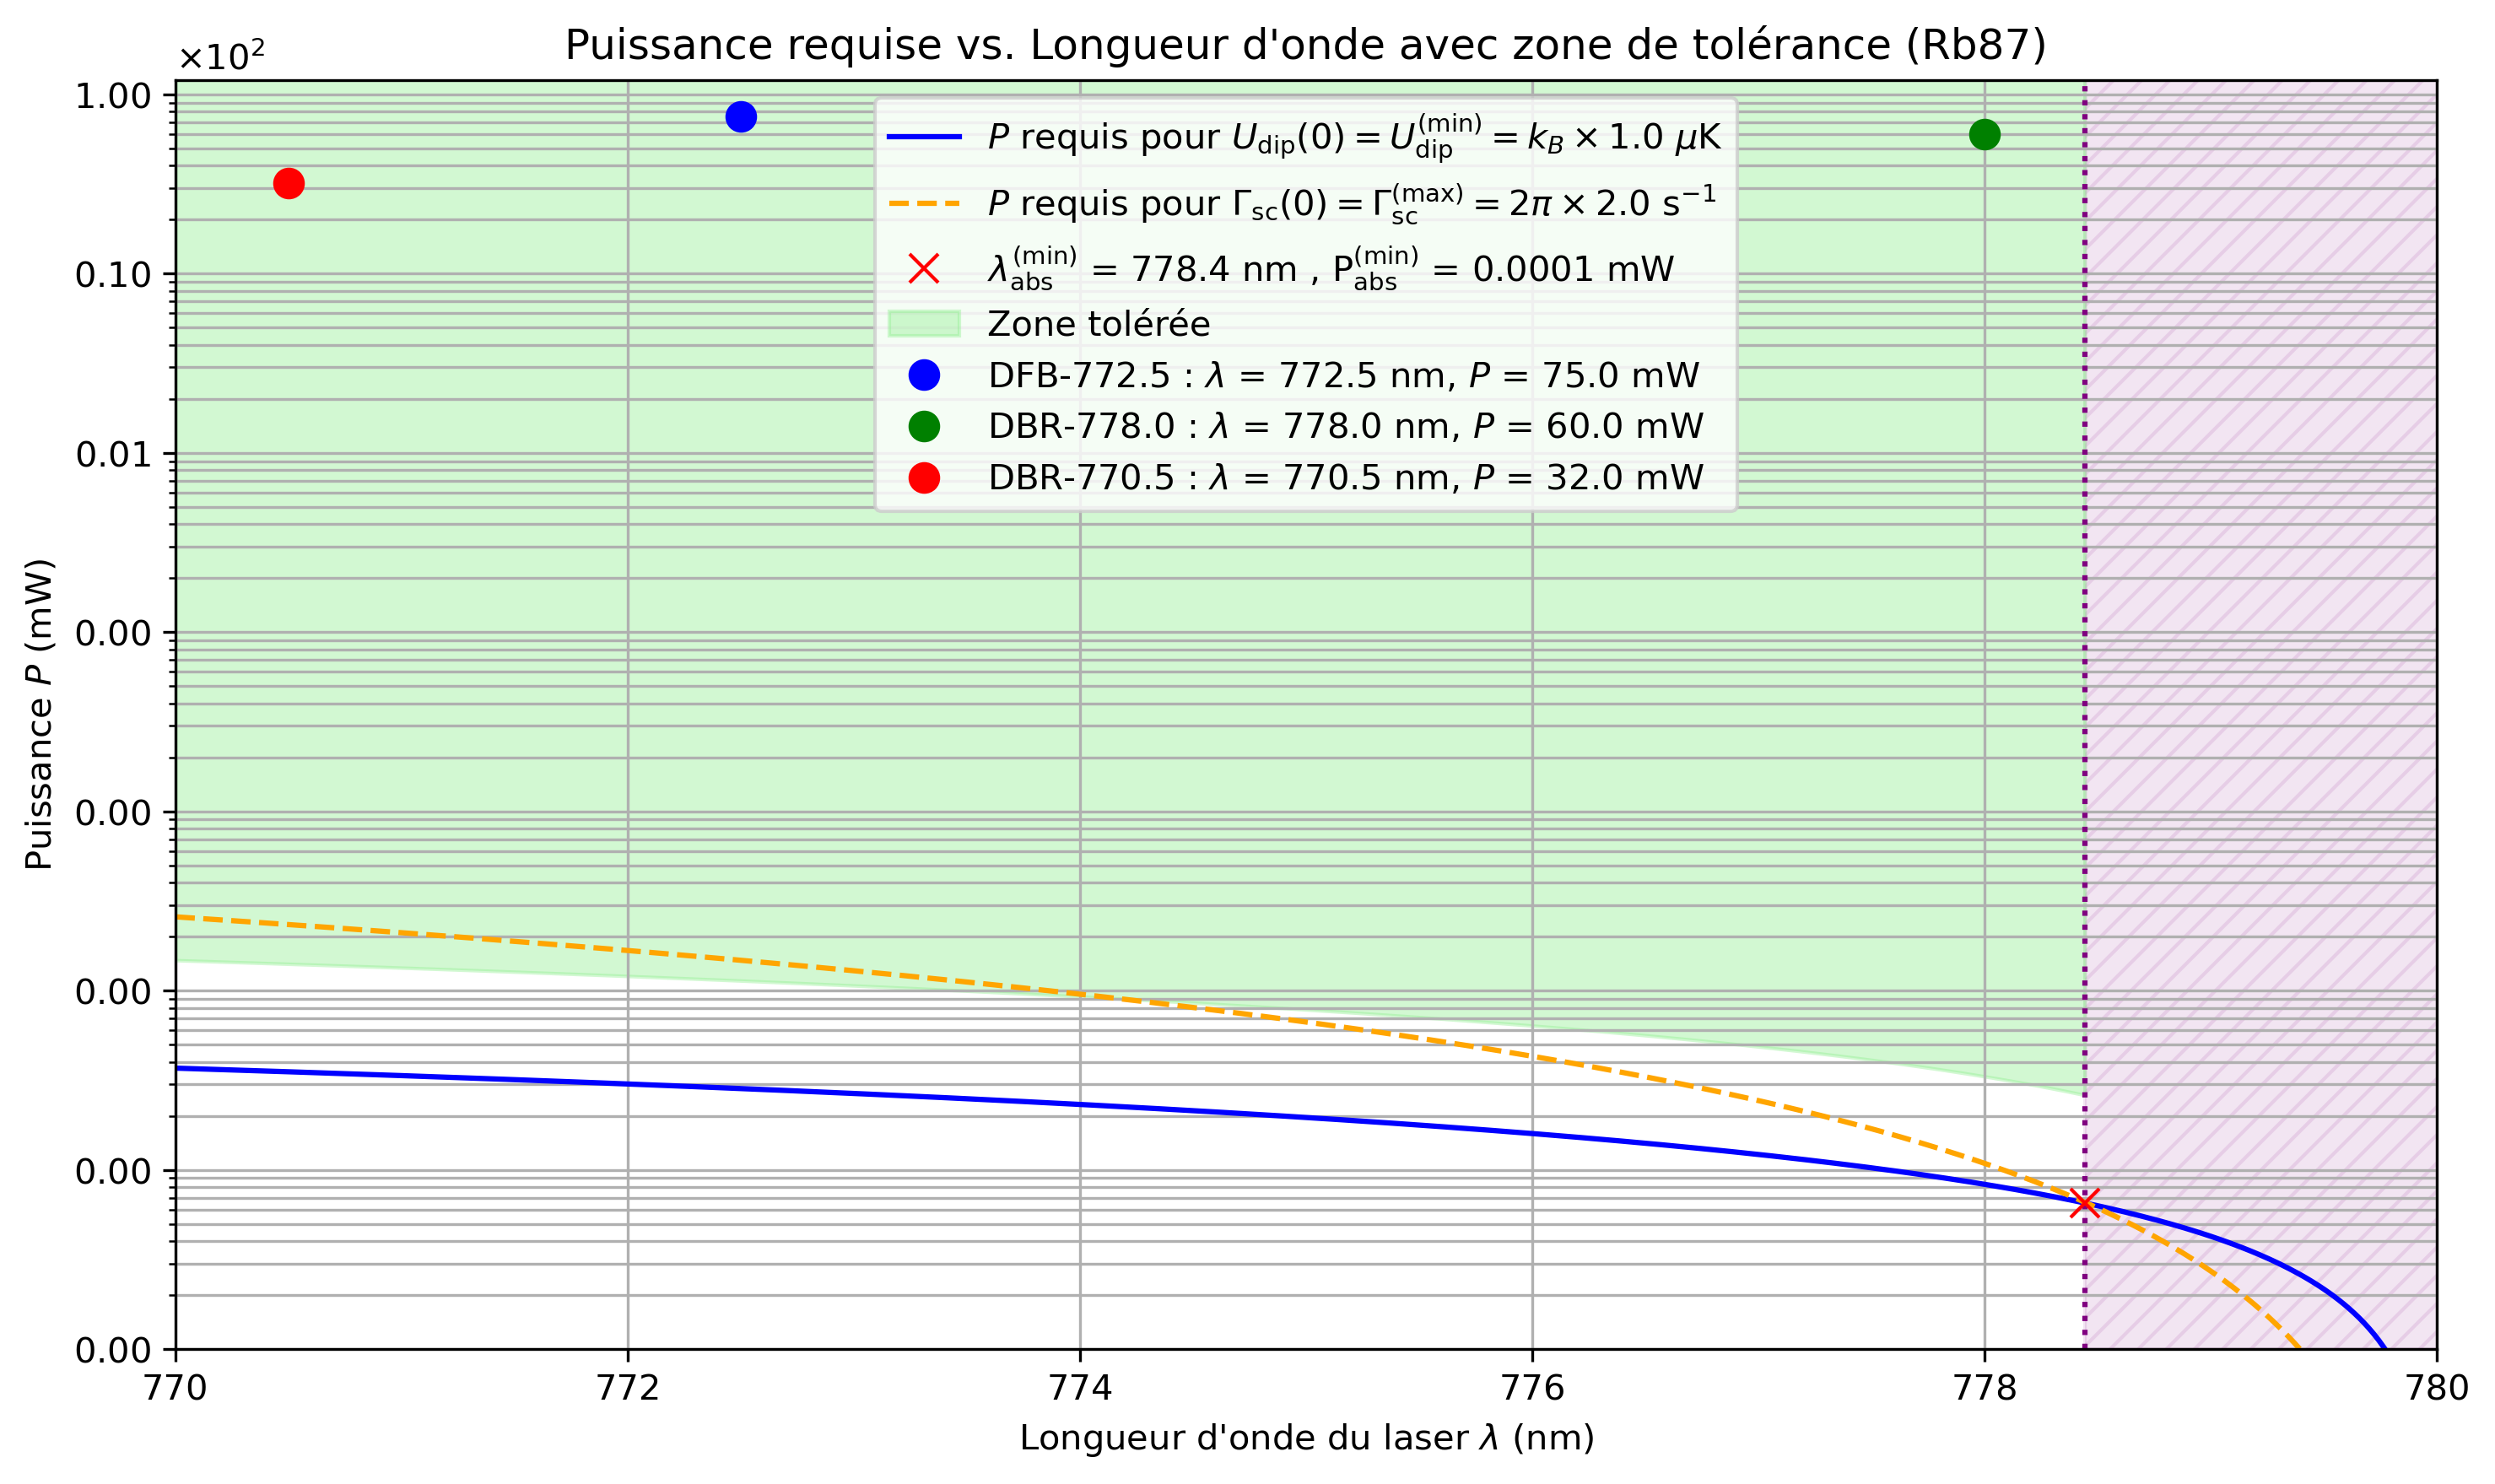
\includegraphics[width=0.7\linewidth]{Dipolaire/Figures/puissance_vs_lambda_log.png}
    \caption{$P^{(min)}(\lambda)$ et $P^{(max)}(\lambda)$}
\end{figure}

L’intersection de ces courbes définit une {\bf zone de faisabilité expérimentale} dans l’espace $(\lambda, P)$. Le croisement des courbes fournit la longueur d’onde maximale admissible :
\begin{eqnarray*}
	\lambda^{(max)}_{abs} \simeq 778.4~nm , \quad P^{(min)}_{abs} \simeq 0.0001 ~ mW
\end{eqnarray*}

Un premier filtrage des sources laser admissibles impose que la longueur d’onde soit inférieure à $\lambda^{(max)}_{\text{abs}}$ et que la puissance disponible dépasse $P^{(min)}_{\text{abs}}$.

%\subsubsection*{Prise en compte des pertes optiques}
%
%L’ensemble des éléments optiques (fibres, lentilles, miroirs, diviseurs de faisceaux) entraîne une perte totale estimée à environ $40–50\%$, ce qui doit être compensé dès le choix des sources laser. En pratique, la puissance utile disponible au niveau des atomes est :
%\[
%P_{utile} = \eta \cdot P_{laser} \quad \mbox{avec} \, \eta = 0.5 .
%\]

\subsubsection*{Prise en compte des pertes optiques}

L’ensemble des éléments optiques traversés par le faisceau — incluant la sortie de fibre, les lentilles de collimation et de focalisation, les miroirs de redirection, les diaphragmes, ainsi que le diviseur de faisceau — induit des pertes cumulées non négligeables. Une estimation réaliste, fondée sur les caractéristiques typiques des composants et l'expérience de montage, indique que les pertes globales s’élèvent à environ $60$ à $75\%$.

Ces pertes doivent être prises en compte dès le dimensionnement initial du système laser, afin de garantir que la puissance effectivement disponible au niveau des atomes soit suffisante pour atteindre les profondeurs de piège souhaitées. En pratique, on modélise cette efficacité par un facteur global $\eta$, défini comme :

\[
P_{\text{utile}} = \eta \cdot P_{\text{laser}}, \quad \text{avec} \quad \eta \simeq 0.25.
\]

Ce coefficient sera utilisé dans la suite pour évaluer les puissances minimales requises des sources laser candidates. Une marge de sécurité est également conservée pour pallier les éventuels désalignements ou dégradations optiques en conditions expérimentales réelles.

%%-------------------------
%Un facteur de sécurité supplémentaire est nécessaire si l’on envisage de moduler l’intensité ou d’utiliser des optiques à densité variable.
%\begin{itemize}
%	\item \textbf{DFB (Distributed Feedback)} à $\lambda = 772.5~\text{nm}$, puissance $P = 75~\text{mW}$ : ce type de diode intègre un réseau de Bragg directement dans la cavité pour assurer une émission monomode stable. C’est un choix très répandu pour les applications atomiques.
%	\item \textbf{DBR (Distributed Bragg Reflector)} à $\lambda = 778.0~\text{nm}$, puissance $P = 60~\text{mW}$ : ici, le réseau est séparé de la région active, ce qui offre une certaine souplesse de réglage, bien que la stabilité spectrale puisse être légèrement inférieure à celle des DFB.
%	\item \textbf{DBR} à $\lambda = 770.5~\text{nm}$, puissance $P = 32~\text{mW}$. 
%\end{itemize}
%
%%\begin{center}
%%\textit{[Ajouter une figure montrant les points expérimentaux des lasers DFB et DBR sur le diagramme $(\lambda, P)$]}
%%\end{center}
%
%\paragraph{Pureté spatiale des sources laser}
%
%Les deux sources laser utilisées dans cette expérience sont de type DBR et DFB, toutes deux pigtaillées sur une fibre monomode à maintien de polarisation (PM780-HP). Bien que des modes transverses d’ordre supérieur puissent, en principe, être présents à l’intérieur de la puce laser, la fibre agit comme un filtre spatial efficace. En effet, la fibre PM780-HP ne guide que le mode fondamental LP$_{01}$ (équivalent au mode gaussien TEM$_{00}$) dans la gamme spectrale utilisée ($770{-}780$ nm). Ainsi, la lumière émise en sortie de fibre est spatialement très pure, avec une fraction de puissance dans le mode TEM$_{00}$ supérieure à $99.5\%$.
%
%Cette configuration garantit que les faisceaux utilisés pour le piégeage optique présentent un profil gaussien stable, propre, et bien adapté à une focalisation contrôlée.
%
%
%Les deux lasers sélectionnés se situent dans la zone admissible définie par les conditions $P^{(min)}(\lambda)$ et $P^{(max)}(\lambda)$. Cela valide leur usage pour construire notre boîte optique bleue destinée au piégeage dipolaire de Rubidium-87.
%
%
%-----------------------------

\subsubsection*{Sources laser utilisées et pureté spatiale}

Trois sources laser ont été sélectionnées pour la réalisation de la boîte optique blue-detuned destinée au piégeage dipolaire du Rubidium-87, dont deux répondent aux conditions de puissance admissibles $P^{(min)}(\lambda)$ et $P^{(max)}(\lambda)$.

\begin{itemize}
    \item \textbf{DFB} à $\lambda = 772.5~\text{nm}$, puissance $P = 75~\text{mW}$.
    \item \textbf{DBR} à $\lambda = 778.0~\text{nm}$, puissance $P = 60~\text{mW}$. 
    \item \textbf{DBR} à $\lambda = 770.5~\text{nm}$, puissance $P = 32~\text{mW}$(,également utilisé pour certaines étapes du montage).
\end{itemize}

\medskip

Le laser DFB (Distributed Feedback) intègre un réseau de Bragg directement dans la région active, ce qui permet un couplage efficace entre la rétroaction optique et le gain, assurant une émission monomode stable tant sur le plan spectral que spatial. Cette architecture confère au DFB une excellente stabilité et une robustesse appréciées en physique atomique.

Le laser DBR (Distributed Bragg Reflector), quant à lui, dispose d’un réseau de Bragg séparé de la région active. Cette configuration offre une plus grande flexibilité dans le réglage de la longueur d’onde, mais entraîne généralement une stabilité spectrale un peu moindre par rapport aux lasers DFB.

\medskip

Ces diodes sont pigtaillées sur des fibres monomodes à maintien de polarisation (type PM780-HP), assurant un profil spatial très pur. En effet, bien que des modes transverses supérieurs puissent être émis par la puce laser, la fibre ne guide que le mode fondamental LP$_{01}$, équivalent au mode gaussien TEM$_{00}$, dans la gamme spectrale $770{-}780~\text{nm}$. Cette configuration agit comme un filtre spatial puissant, garantissant une sortie de faisceau gaussien avec une pureté supérieure à $99.5\%$ en puissance.

\medskip

Cette haute pureté spatiale est cruciale pour obtenir une focalisation optimale et des gradients de champ suffisamment intenses dans la zone de piégeage, tout en minimisant les pertes optiques et les effets parasites liés à la présence de modes non fondamentaux.

Enfin, les troix lasers  se situent dans la zone de tolérence définie par les conditions sur la puissance minimale et maximale en fonction de la longueur d’onde, validant leur adéquation pour la construction de notre boîte optique blue-detuned.

\medskip

Avec un waist de $w_0 = 1~\mu\text{m}$, les puissances minimales requises pour satisfaire les conditions $U_{dip}^{(min)}$ et $\Gamma_{sp}^{(max)}$ sont extrêmement faibles : environ $1.1~\mu\text{W}$ pour la DFB à $772.5~\text{nm}$, $0.3~\mu\text{W}$ pour la DBR à $778.0~\text{nm}$, et $1.4~\mu\text{W}$ pour la DBR à $770.5~\text{nm}$. Ces valeurs sont très largement inférieures aux puissances disponibles pour chacun de ces lasers, même en tenant compte des pertes optiques, ce qui confirme la faisabilité expérimentale du dispositif.

\paragraph{Choix initial du waist.}

Lors de la sélection initiale des lasers, une hypothèse conservative a été faite en supposant un waist focalisé de $w_0 = 300~\text{nm}$ au niveau des atomes. Ce choix était motivé par une estimation de l’échelle typique des variations du potentiel dans la boîte optique, et visait à garantir une intensité suffisante à petite échelle.

\medskip

Avec le recul, cette valeur s’est avérée trop pessimiste. Le système optique finalement mis en place permet des waists plus larges (de l’ordre du micron), mieux adaptés à la géométrie expérimentale et aux contraintes de focalisation. Cette hypothèse initialement sous-estimée a toutefois eu pour effet bénéfique de conduire à une surévaluation des puissances requises, fournissant une marge de sécurité bienvenue dans le dimensionnement des sources laser.

\medskip

Avec un waist de $w_0 = 300~\mu\text{m}$, les puissances minimales requises augmentent considérablement en raison de la baisse d’intensité au centre du faisceau. On obtient alors des puissances nécessaires de l’ordre de $102~\text{mW}$ pour la DFB à $772.5~\text{nm}$, $30~\text{mW}$ pour la DBR à $778.0~\text{nm}$, et $127~\text{mW}$ pour la DBR à $770.5~\text{nm}$. Seul le laser à $778.0~\text{nm}$ satisfait cette condition sans amplification supplémentaire. En revanche, les deux autres lasers se trouvent sous-dimensionnés dans ce scénario, ce qui justifie le recours à un amplificateur optique dans le cas du laser à $770.5~\text{nm}$.

\medskip

Ce constat a notamment motivé l’ajout d’un amplificateur optique (TA — Tapered Amplifier) en sortie du laser à $770.5~\text{nm}$, afin de compenser la puissance disponible limitée et garantir des conditions de piégeage satisfaisantes malgré les pertes optiques du système.

\begin{center}
\textit{[Photos laser à $770.5~\text{nm}$ ]}
\end{center}


\subsection{Amplification par Tapered Amplifier (TA)}

\subsubsection*{Principe et motivation}

Afin de compenser le déficit de puissance du laser DBR à $770.5~\text{nm}$ — notamment dans le scénario initialement envisagé avec un waist focalisé important — un amplificateur optique de type \textit{Tapered Amplifier} (TA) a été ajouté en aval de la source laser.

Un TA est un semi-conducteur optique amplificateur non résonant, composé d'une région d'entrée étroite (guidée) et d'une région de sortie évasée (tapered), permettant d'amplifier efficacement un faisceau monomode tout en conservant un profil spatial de bonne qualité. Contrairement aux lasers, le TA n'oscille pas par lui-même : il agit uniquement sur un signal incident (seed). Il peut amplifier des puissances faibles (quelques mW) en entrée jusqu’à plusieurs centaines de mW, voire au-delà, en sortie.

Ce dispositif est particulièrement adapté aux expériences de piégeage optique, où une puissance laser relativement élevée est nécessaire tout en maintenant une bonne qualité spatiale.

\subsubsection*{Contraintes et précautions}

L'utilisation d’un TA s’accompagne de plusieurs contraintes expérimentales importantes :

\begin{itemize}[label=$\bullet$]
    \item \textbf{Sensibilité aux rétro-réflexions :} la puce du TA ne supporte pas les retours optiques parasites, qui peuvent entraîner des instabilités, des dégradations de performance, voire endommager le composant. Un \textbf{isolateur optique} est donc placé en sortie pour bloquer tout retour de lumière vers le TA.
    
    \item \textbf{Sensibilité à l’alignement :} une injection efficace du faisceau dans la zone guidée d’entrée du TA requiert un alignement très précis. Celui-ci est réalisé à l’aide de deux miroirs montés sur des supports à réglage fin, offrant 4 degrés de liberté (translations X–Y, inclinaisons $\theta_x$, $\theta_y$).
    
    \item \textbf{Émission multi-modes en sortie :} malgré une injection monomode, la sortie du TA présente parfois plusieurs lobes d’intensité dus à la géométrie évasée. Un diaphragme ou une \textbf{pinhole} de $50~\mu$m (à ajuster selon le profil observé) est donc utilisé pour filtrer spatialement le mode fondamental TEM$_{00}$.
\end{itemize}

\subsubsection*{Mise en œuvre expérimentale}

Le schéma global de l’amplification est présenté sur la figure~\ref{fig:TA_setup} (non incluse ici).

\begin{itemize}[label=$\triangleright$]
    \item \textbf{Laser seed :} le laser DBR à $770.5~\text{nm}$ est stabilisé en température et en courant à l’aide du contrôleur Thorlabs ITC-510, et injecté dans le TA à l’aide d’une optique de couplage sur table optique.
    
    \item \textbf{Boîtier de protection et régulation thermique :} le TA est installé dans un boîtier métallique maison, conçu pour assurer à la fois une protection mécanique et une stabilité thermique. Ce boîtier intègre un module Peltier et une thermistance pour la régulation active de la température, pilotés par un contrôleur thermique (Arrow OEM). L’ensemble est alimenté par une alimentation dédiée (Delta Electronics), garantissant un fonctionnement stable du système de refroidissement. Cette stabilisation thermique est cruciale pour limiter les dérives du TA et préserver la qualité spatiale du faisceau amplifié.

    \item \textbf{Filtrage spatial :} une pinhole positionnée en sortie du TA permet de sélectionner le mode spatial fondamental.

    \item \textbf{Isolateur optique :} un isolateur optique est placé immédiatement après le TA pour éviter tout retour de lumière vers la puce.

    \item \textbf{Modulation de puissance :} un modulateur acousto-optique (AOM) est inséré juste avant la fibre optique, permettant de couper la lumière à la demande (switch rapide) ou de moduler dynamiquement l’intensité laser. Cela permet un contrôle fin de l’illumination au niveau des atomes.
    
    \item \textbf{Mesure de puissance :} une photodiode ou un power meter placé après l’AOM permet de calibrer précisément la puissance en fonction du courant injecté dans le TA, et de corriger les effets d’instabilité si besoin.
\end{itemize}

\subsubsection*{Caractérisation et performance}

La diode laser et le Tapered Amplifier (TA) sont asservis à une température stable de $25^\circ$C. Une courbe de puissance de sortie du TA en fonction du courant injecté a été mesurée (voir figure~\ref{fig:Puissance_TA}), avec la diode laser fonctionnant à $25^\circ$C et délivrant une puissance maximale d’environ $31.2\,\text{mW}$, tandis que le TA est testé jusqu’à un courant d’injection de $2.5\,\text{A}$.

\begin{figure}[H]
    \centering
    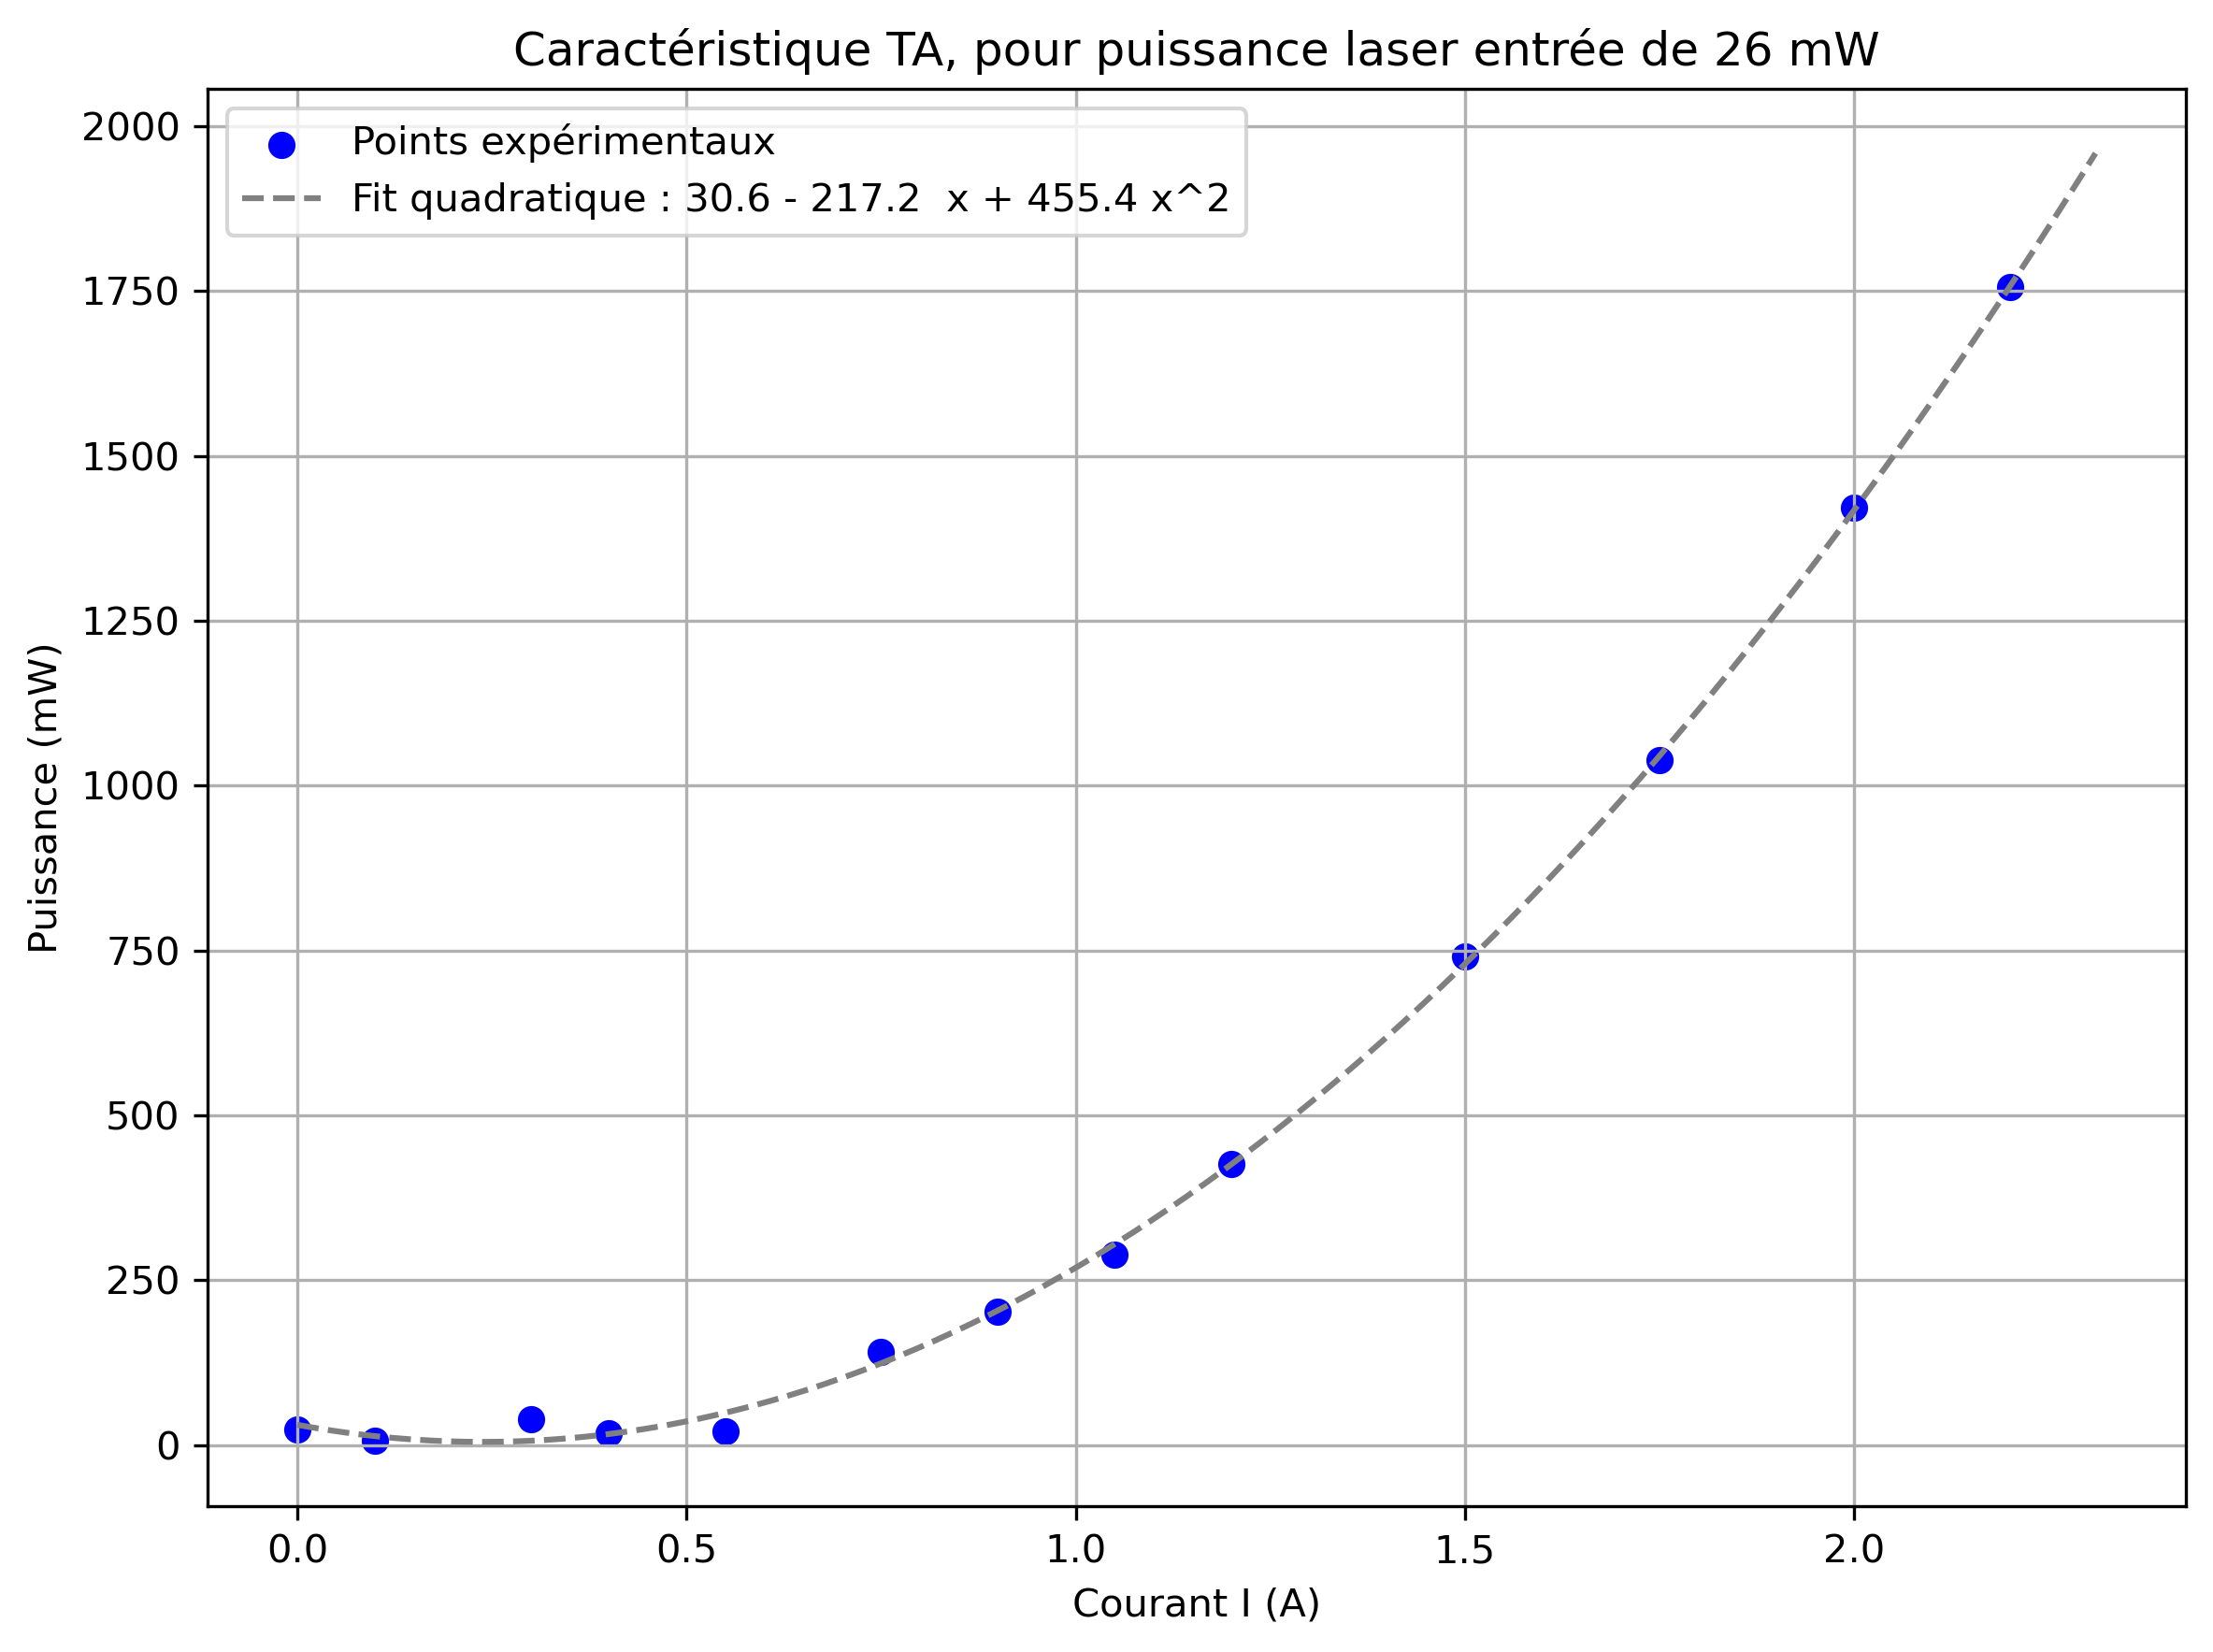
\includegraphics[width=0.7\linewidth]{Dipolaire/Figures/Puissance_TA.png}
    \caption{Puissance de sortie du Tapered Amplifier (TA) en fonction du courant d’injection, pour une puissance d’entrée provenant de la diode laser fixée à 25 mW.}
    \label{fig:Puissance_TA}
\end{figure}

Afin d’éviter une dégradation prématurée des composants, il a été choisi de ne pas les faire fonctionner à leurs limites maximales. La diode laser est ainsi réglée pour fournir une puissance d’environ $25\,\text{mW}$ (courant $I_{\text{diode}} = 150.6\,\text{mA}$) et le TA est exploité avec un courant d’environ $1.5\,\text{A}$. Cette configuration assure un bon compromis entre puissance de sortie et longévité des dispositifs, tout en garantissant une amplification stable et un profil spatial préservé.


Pour un courant d’injection de $1.5\,\text{A}$ dans le TA, la puissance mesurée en sortie, après passage dans le modulateur acousto-optique (AOM), atteint environ $62\,\text{mW}$. 

L’AOM génère plusieurs ordres de diffraction : le mode zéro (non diffracté), les modes $\pm 1$, etc. Afin d’optimiser le transfert d’énergie dans un mode diffracté souhaité (par exemple le premier ordre $\pm 1$), le cristal AOM a été ajusté finement en rotation. Ce réglage permet de maximiser la puissance dans ce mode non nul.

Le faisceau correspondant à ce mode diffracté, qui concentre la majorité de la puissance utile, est ensuite injecté dans une fibre monomode à maintien de polarisation. 

Ainsi, l’AOM est configuré de manière à transférer efficacement la puissance vers le mode diffracté utile, avec une puissance d’environ $62\,\text{mW}$ disponible à l'entée de la fibre, garantissant une qualité spatiale et une polarisation stables pour l’expérience.


Le système ainsi mis en place permet d’obtenir, de manière stable, une puissance suffisante en sortie pour alimenter la fibre de piégeage, même en tenant compte des pertes optiques du système.



%Le projet est de fais une boite en utilisant un potentielle dipolaire électique induite par un laser dans la longeur d'onde et decaler dans le blue ($\Delta > 0 $) par raport au transition D1 et D2 des atomes de Rubidium97. 
%On partie d'un systeme d'atome froid , unidimentionelle. On fait dest faiseaux dipolaires à diferrent postions. Les atomes seron confiné dans la zone entre les faiseaux. 
%
%\vspace{1em}
%% INSERTION FIGURE
%\begin{center}
%\textit{[Insérer ici schéma des deux faiseaux avec les atomes au milieux]}
%\end{center}
%
%Maintent , il faux caracteriser ces faisceaux. Dans un premier tempst on a avus Il y a 2 parametre a prend en compte , les potentiel pic aux niveau des atomes $U_{dip}(0)$ , qui impluence la profondeur du puit , les Taux d'emition spontané pic $\Gamma_{sp}(0)$ qui influence .... .
%On veux que $U_{dip}(0)$ soit siperieur a une maleur minimur , que pour les calcule futur on noterar $U_{dip}^{(min)}(0)$ , cette valeur serais de $1 k_B \times \mu K $ (pour .... peut etre une raison dans la literature ) , et puis on impose que pour $x^\ast$ tel que $U_{dip}(x^\ast)= U_{dip}(0)/2$ , $\Gamma_{dip}(x^\ast)$ imferieur à une valeur maximume de $2\pi \times 1 s^{-1}$. En remarquant les potentielle $U_{dip}(\vec{r})$  et le taux de difusions $\Gamma_{sp}(\vec{r})$ sont proportionnelle à l'intentité $I(\vec{r})$ , on constante que cette dernier condition est equivalente à $\Gamma_{sp}(0) \leq \Gamma_{sp}^{(max)}(0) = 2\pi \times 2 ~s^{-1}$. 
%
%\paragraph{Ratio figure de mérite : potentiel / diffusion}
%Il est utile de comparer le potentiel conservatif $U_{dip}$ au taux de diffusion $\Gamma_{sc}$ pour quantifier l’efficacité du piégeage :
%\begin{eqnarray*}
%	\frac{U_{dip}(\vec{r})}{\hbar \Gamma_{sc}(\vec{r})} = \frac{1}{\Gamma} \frac{ \left( \frac{ 1}{ 3 \Delta_1} + \frac{2 }{ 3 \Delta_2}  \right )}{\left( \frac{ 1}{ 3 \Delta_1^2} + \frac{2 }{ 3 \Delta_2^2}  \right )} \geq \frac{U_{dip}^{(min)}(0)}{\hbar \Gamma_{sc}^{(max)}(0)}.
%\end{eqnarray*}
%Ce rapport est homogène à une {\bf fréquence}, et correspond à l’inverse d’un {\bf temps caractéristique} entre deux événements de diffusion. Plus il est grand, plus le piégeage est efficace avec peu d’échauffement. Il permet également d’estimer :
%\begin{itemize}[label=$\bullet$]
%	\item La {\bf longueur d’onde optimale} (balancement entre profondeur de piège et faible taux de diffusion),
%	\item La {\bf puissance minimale nécessaire}  à une barrière donnée,
%	\item La {\bf faisabilité}  d’un piège blue-detuned (ou red-detuned).
%\end{itemize}
%
%Un calcule numérique , nous dit que avec cette condition on doit chercher des laser avec des longueur d'onde inferieux-r a la longeur d'onde max $\lambda^{(max)} = 778,4 ~ nm$.
%
%(	\item La {\bf puissance minimale nécessaire}  à une barrière donnée,
%	\item La {\bf faisabilité}  d’un piège blue-detuned (ou red-detuned).
%comment ????? 
%) 
%
%c'est une premier information mais les faiseaux sera gaussien avec un waist $w_0$ des quelque centaine de nm (car ....) . 
%Avec $I(0) = \frac{2P}{\pi w_0^2}$ , avec $P$ la puissance du laser. On deux condition qui bornent la puissance du laser pour un longeur du laser $\lambda$ d'on donné : 
%
%\begin{eqnarray*}
%	 \underbrace{U_{dip}^{(min)}(0) \frac{\pi w_0^2}{2} \frac{8 I_{sat}}{\Gamma^2}\left/\left( \frac{ 1}{ 3 \Delta_1} + \frac{2 }{ 3 \Delta_2}  \right ) \right.}_{P^{(min)}(\lambda)}  \leq P(\lambda) \leq \underbrace{ \Gamma_{sc}^{(max)}(0) \frac{\pi w_0^2}{2} \frac{8 I_{sat}}{\Gamma^3}\left/\left( \frac{ 1}{ 3 \Delta_1^2} + \frac{2 }{ 3 \Delta_2^2}  \right )\right.}_{ P^{(max)}(\lambda)} 
%\end{eqnarray*}
%
%\vspace{1em}
%% INSERTION FIGURE
%\begin{center}
%\textit{[Insérer ici schéma des courbe P ]}
%\end{center}
%
%Sur cette figure on a representer cest deux courbe , P^{(min)} , P^{(max)} , une croix rouge represente là ous les deux courbe se croise , la cordonnée $(\lambda^{(max)} , P^{(min)}_{abs})$. Un filtrege grossier pour le chois de nos laser est un laser avec une longeur d'onde inferieur a $\lambda^{(max)} = ... $ et une puicane superieur à $P^{(min)}_{abs} = ...$.
%
%LA puiscent du laser au niveau des atomes doit etre pour une longeur d'onde donnet etre danst les zone etre les deux courbe.
%J'estimes que les perter du au optique est de ???\% (fibre optique , miroire , lentille et deboublement du du faisseaux  ) . Et biens sur si la puissance est trop brande on peut ajouter des densité opitique donc , avec cette marge de ???\% je choix des lazer doit etre dans la zone bleu sur la figure .
%J'ai selectionner 2 laser avec les cacteristique suivante :
%
%\begin{itemize}
%	\item DFB de longueur d'onde $772.5 ~nm$ et de Puissance $75.0~ mW$ ( les point rouge sur la figure  
%	\item DBR de longueur d'onde $778.0 ~nm$ et de Puissance $60.0~ mW$ ( les point blue sur la figure 	
%\end{itemize}














%\subsubsection{Quelle longueur d'onde ?}





